\documentclass[12pt]{aghdpl}

\usepackage[english,polish]{babel}

% Użyj polskiego łamania wyrazów (zamiast domyślnego angielskiego).
\usepackage{polski}

\usepackage[utf8]{inputenc}

% dodatkowe pakiety

\usepackage{mathtools}
\usepackage{amsfonts}
\usepackage{amsmath}
\usepackage{amsthm}

% --- < bibliografia > ---

\usepackage[
style=numeric,
sorting=none,
%
% Zastosuj styl wpisu bibliograficznego właściwy językowi publikacji.
language=autobib,
autolang=other,
% Zapisuj datę dostępu do strony WWW w formacie RRRR-MM-DD.
urldate=iso8601,
% Nie dodawaj numerów stron, na których występuje cytowanie.
backref=false,
% Podawaj ISBN.
isbn=true,
% Nie podawaj URL-i, o ile nie jest to konieczne.
url=false,
%
% Ustawienia związane z polskimi normami dla bibliografii.
maxbibnames=3,
% Jeżeli używamy BibTeXa:
backend=bibtex
]{biblatex}

\usepackage{csquotes}
% Ponieważ `csquotes` nie posiada polskiego stylu, można skorzystać z mocno zbliżonego stylu chorwackiego.
\DeclareQuoteAlias{croatian}{polish}

\addbibresource{bibliografia.bib}

% Nie wyświetlaj wybranych pól.
%\AtEveryBibitem{\clearfield{note}}


% ------------------------
% --- < listingi > ---

% Użyj czcionki kroju Courier.
\usepackage{courier}

\usepackage{listings}
\lstloadlanguages{TeX}

\lstset{
	literate={ą}{{\k{a}}}1
           {ć}{{\'c}}1
           {ę}{{\k{e}}}1
           {ó}{{\'o}}1
           {ń}{{\'n}}1
           {ł}{{\l{}}}1
           {ś}{{\'s}}1
           {ź}{{\'z}}1
           {ż}{{\.z}}1
           {Ą}{{\k{A}}}1
           {Ć}{{\'C}}1
           {Ę}{{\k{E}}}1
           {Ó}{{\'O}}1
           {Ń}{{\'N}}1
           {Ł}{{\L{}}}1
           {Ś}{{\'S}}1
           {Ź}{{\'Z}}1
           {Ż}{{\.Z}}1,
	basicstyle=\footnotesize\ttfamily,
}

% ------------------------

\AtBeginDocument{
	\renewcommand{\tablename}{Tabela}
	\renewcommand{\figurename}{Rys.}
}

% ------------------------
% --- < tabele > ---

\usepackage{array}
\usepackage{tabularx}
\usepackage{multirow}
\usepackage{booktabs}
\usepackage{makecell}
\usepackage[flushleft]{threeparttable}

% defines the X column to use m (\parbox[c]) instead of p (`parbox[t]`)
\newcolumntype{C}[1]{>{\hsize=#1\hsize\centering\arraybackslash}X}


%---------------------------------------------------------------------------

\author{Amadeusz Hercog}
\shortauthor{A. Hercog}

%\titlePL{Przygotowanie bardzo długiej i pasjonującej pracy dyplomowej w~systemie~\LaTeX}
%\titleEN{Preparation of a very long and fascinating bachelor or master thesis in \LaTeX}

\titlePL{Wykorzystanie algorytmu sztucznej inteligencji do rozwiązania problemu optymalnego wyboru ścieżki lub wyjścia ewakuacyjnego}
\titleEN{}


\shorttitlePL{Rozwiązanie problemu optymalnego wyboru ścieżki lub wyjścia ewakuacyjnego} % skrócona wersja tytułu jeśli jest bardzo długi
\shorttitleEN{}

\thesistype{Praca dyplomowa inżynierska}
%\thesistype{Master of Science Thesis}

\supervisor{mgr. inż. Robert Lubaś}
%\supervisor{Marcin Szpyrka PhD, DSc}

\degreeprogramme{Informatyka stosowana}
%\degreeprogramme{Computer Science}

\department{Wydział Informatyki Stosowanej}
%\department{Department of Applied Computer Science}

\faculty{Wydział Fizyki i Informatyki}
%\faculty{Faculty of Electrical Engineering, Automatics, Computer Science and Biomedical Engineering}

\acknowledgements{Serdecznie dziękuję mojemu promotorowi Robertowi Lubaś za pomoc w wykonaniu pracy inżynierskiej.}

\setlength{\cftsecnumwidth}{10mm}

%---------------------------------------------------------------------------
\setcounter{secnumdepth}{4}
\brokenpenalty=10000\relax

% arial
\renewcommand{\rmdefault}{phv}
\renewcommand{\sfdefault}{phv}

% wyłączenie łamania słów i justowanie
\usepackage[none]{hyphenat}
\sloppy

% wcięcie na pierwszych liniach rozdziałów
\usepackage{indentfirst}

% klikalne linki
\usepackage[colorlinks, linkcolor=blue]{hyperref}

% dane dokumentu
\title{Wykorzystanie algorytmu sztucznej inteligencji do rozwiązania problemu optymalnego wyboru ścieżki lub wyjścia ewakuacyjnego}
\author{Amadeusz Hercog}
\date{21 listopada 2018}

% ładnie wystylizowana tabela
\usepackage[table, svgnames]{xcolor} \usepackage{array}
\usepackage{etoolbox}

\definecolor{table_header_color}{HTML}{B0BEC5}
\definecolor{even_row_color}{HTML}{EEEEEE}

\newenvironment{tightcenter}{
  \setlength\topsep{0pt}
  \setlength\parskip{0pt}
  \begin{center}
}{
  \end{center}
}

\newenvironment{mytabular}{\rowcolors{1}{\ifnumless{\rownum}{2}{table_header_color}{even_row_color}}{}\begin{tightcenter}\tabular}{\endtabular\end{tightcenter}}

% kolumna z zawijaniem
\newcolumntype{L}{>{\centering\arraybackslash}m{3cm}}

% centrowanie nagłówków
\captionsetup{justification=centering}

% wykresy w sekcjach w których sie je zdefiniowało
\usepackage[section]{placeins}

\begin{document}
	\titlepages
	
	\chapter{Wstęp}
	\textit{W tym rozdziale zostanie opisane podłoże historyczne, cel i jego założenia projektu. Zaprezentowane zostanie proponowane rozwiązanie postawionego problemu oraz technologie do tego użyte.}
	
		\section{Geneza projektu}	
		W dzisiejszym świecie kładziony jest nacisk na projektowanie budynków użytku publicznego tak, aby zapewnić możliwie największe bezpieczeństwo ludzi, którzy będą z nich korzystali. Jednakże, jednocześnie wymagane jest aby takie budynki były także funkcjonalne - na przykład odpowiednie zaplanowanie podziału na pomieszczenia. Z tych powodów konieczne jest wyznaczenie ścieżek oraz wyjść ewakuacyjnych przewidzianych w taki sposób, aby ewakuacja ludzi odbyła się w sposób sprawny a jednocześnie, aby zachować wysoką funkcjonalność budynku.
		
		Dziedzina informatyki, jaką jest uczenie maszynowe przez kilka ostatnich lat zyskała sporą popularność. Metody z tej dziedziny potrafią rozwiązywać problemy, które dotychczas były nierozwiązywalne za pomocą innych metod. Jednym z takich problemów jest uczenie się wzorca na podstawie zbioru danych oraz jego generalizacja. Daje to duże możliwości w takich zadaniach, gdzie potrzebujemy narzędzia potrafiącego symulować ruch ludzi na podstawie wcześniej nauczonych wzorców. Przykładowo niektóre gry komputerowe, jak seria \textit{Halo}, w których zachowania postaci muszą być jak najbardziej naturalne, więc są trenowane na podstawie danych rzeczywistych.
		
		Rozwiązanie problemu optymalnego wyboru ścieżki lub wyjścia ewakuacyjnego dałoby odpowiedź jaki jest najkrótszy czas ewakuacji całego budynku, co daje informacje o tym, czy budynek jest dobrze zaprojektowany pod kątem parametrów transportowych pieszych.
	
		\section{Cel projektu}	
		 W ramach pracy autor postawił sobie następujący problem - rozwiązanie problemu optymalizacji wyboru ścieżki lub wyjścia ewakuacyjnego ludzi w budynku. Co więcej, w związku z wcześniejszym doświadczeniem z tematem uczenia maszynowego (ang. machine learning), autor postanowił rozwiązać ten problem za pomocą właśnie tych technik.
		
		\section{Użyte technologie oraz programy}
		Wszystkie obliczenia oraz rysowanie wykresów zostały zrealizowane w języku programowania \textbf{Python} w wersji 3.6 przy użyciu bibliotek:
		\begin{itemize}
			\item \textbf{NumPy} - służąca do obliczeń numerycznych,
			\item \textbf{Pandas} - służąca łatwiejszemu zarządzaniu duzą ilością danych,
			\item \textbf{Matplotlib} - służąca do rysowania wykresów,
			\item \textbf{Tensorflow} - używana do głębokiego uczenia maszynowego.
		\end{itemize}
		
		Opiekun pracy udostępnił oprogramowanie - symulator \textbf{PSP} \textit{(Pederastian Simulation Project)}, który daje możliwość symulacji ruchu pieszych w budynku. Jest on opisany szerzej w rozdziale~\ref{sekcja_psp}.
		
	\chapter{Wstęp teoretyczny}
	\textit{W tym rozdziale rozróżniono typy algorytmów uczenia maszynowego. Omówiono koncepcję Perceptronu. Przedstawiono także jedną z metod optymalizacji jaką jest metoda gradientu prostego. Ukazano w jaki sposób za pomocą tej metody można zoptymalizować wyjścia modelu uczenia maszynowego na podstawie jej wejść.}
	
		\section{Typy modeli uczenia maszynowego}
		Uczenie maszynowe jest to termin określający całą gamę sposobów rozwiązywania problemów, które przy tradycyjnych metodach byłyby niemożliwe do rozwiązania lub skrajnie niewydajne obliczeniowo. Wyróżniane są 4 typy algorytmów uczenia maszynowego ze względu na sposób rozwiązywania przez nie problemu 	\cite{types_of_machine_learning_algorithms}:
		\begin{itemize}
		\item \textbf{Uczenie z nadzorem} (ang. supervised learning) - algorytmy, do których danymi wejściowymi są zestawy cech i ich etykiety oznaczające do jakiej kategorii przynależy dana próbka. Tak nauczony model potrafi przewidzieć etykiety dla nowych zestawów cech.
		\item \textbf{Uczenie bez nadzoru} (ang. unsupervised learning) - typ algorytmów, do których dostarczane są tylko dane w postaci zbioru cech. Algorytm ma za zadanie sklasteryzować dane na podstawie podobieństw między nimi.
		\item \textbf{Uczenie pół-nadzorowane} (ang. semi-supervised learning) - te algorytmy są połączeniem algorytmów \textit{uczenia z nadzorem} oraz \textit{uczenia bez nadzoru}. Przyjmują one dane, których tylko część jest oznaczona etykietami - na nich uczą się klasyfikacji, a na pozostałych (nieoznaczonych) - klasteryzacji.
		\item \textbf{Uczenie ze wzmacnianiem} (ang. reinforcement learning) - są zupełnie odmienne od pozostałych typów algorytmów, gdyż nie uczą się na podstawie wcześniej przygotowanych danych wejściowych. Służą one do takich zadań, gdzie na podstawie obserwacji interakcji z pewnym środowiskiem, algorytm się uczy podejmowania najbardziej opłacalnych akcji. Algorytmy te zbierają one dane na bieżąco, cały czas się na nich ucząc.
		\end{itemize}
		
		\section{Perceptron - model regresji}
		Głównymi zadaniami, do których używane są algorytmy \textit{Uczenia z nadzorem} są regresja i klasyfikacja - mając dane wejściowe i ich etykiety, algorytmy te dają możliwość nauczenia modelu powiązań pomiędzy nimi. Regresja przewiduje etykiety, które są wartościami ciągłymi a klasyfikacja - etykiety binarne (\textit{czy to jest pies?}, \textit{czy to jest kot?} i tym podobne).
		
			\subsection{Opis Perceptronu}
			Najprostszym modelem pozwalającym na regresję oraz na klasyfikację jest \textbf{Perceptron} \cite{perceptron_1}\cite{perceptron_2}. Jest on przykładem jednowarstwowej sieci neuronowej. Posiada on zestaw neuronów wejściowych, każdy odpowiadający pojedynczej danej wejściowej. Składa się on także z jednego lub wielu niezależnych neuronów wyjściowych. Każdy z nich jest połączony ze wszystkimi neuronami wejściowymi za pomocą krawędzi posiadających wagi - definiują one jak duży wpływ na wyjście ma każda dana wejściowa. Jeśli wyrazimy:
			\begin{itemize}
			\item wektor wejść jako \textit{X},
			\item wektor wyjść jako \textit{Y},
			\item macierz wag jako \textit{N},
			\item \textbf{funkcję aktywacji} jako $\sigma$ - szerzej opisana w sekcji \ref{parametry_perceptronu}
			\end{itemize}
			to zachodzi równanie:
			
			\begin{equation}
			Y=\sigma(NX)
			\end{equation}
		
			Budowa Perceptronu z jednym neuronem wyjściowym (oznaczonym jako \textit{a}) jest widoczna na rysunku \ref{fig: budowa_perceptronu}\footnote{\url{https://pythonmachinelearning.pro/perceptrons-the-first-neural-networks/}}.
	
			\begin{figure}[h]
		 		\begin{tightcenter}
		 			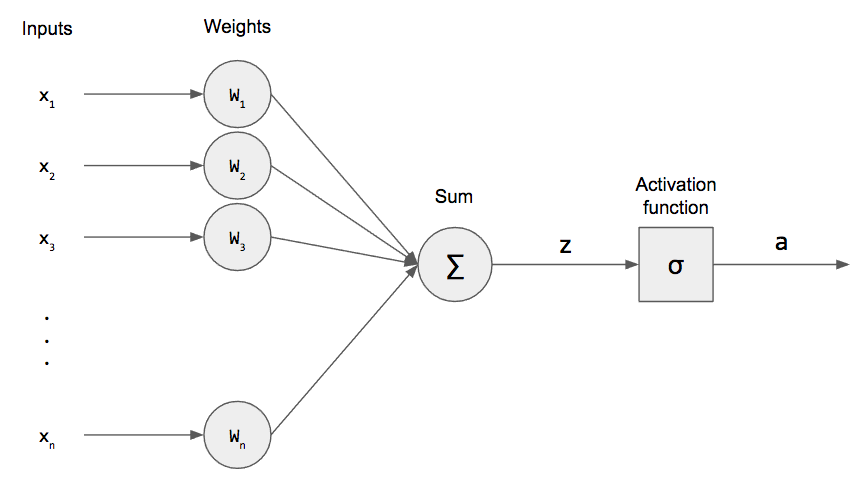
\includegraphics[width = \linewidth]{rysunki/perceptron.png}
				\end{tightcenter}	 			
		 			
	 			\caption{Budowa Perceptronu z jednym neuronem wyjściowym.}
				\label{fig: budowa_perceptronu}
			\end{figure}

			\subsection{Parametry Perceptronu} \label{parametry_perceptronu}
			Modele \textit{Perceptron} posiadają pewien zestaw parametrów, który wpływa na proces uczenia w różny sposób. Nie ma uniwersalnego sposobu ich wyboru co oznacza, że proces ich doboru jest najczęściej serią testów z różnymi ich kombinacjami. Wszystkie parametry opisane w tej sekcji tyczą się modelu \textit{Perceptron} jak i wielowarstwowych sieci neuronowych.
			
			Pierwszym z parametrów jest funkcja aktywacji - wprowadza ona nieliniowość danych w sieci \cite{activation_functions_1}\cite{activation_functions_2}. Służy ona także do ograniczania zakresu danych, najczęściej do przedziału (-1, 1). Wybrane z nich to:
			\begin{itemize}
			
			\item\textbf{Sigmoid} - stosowana często przy klasyfikacji, mająca wzór widoczny na równaniu \ref{rownanie_sigmoid},
			\begin{equation} \label{rownanie_sigmoid}
			\sigma(x) = \frac{1}{1 + e^{-x}}
			\end{equation}
			
			\item\textbf{ReLU (Rectified linear unit)} - ze wzorem widocznym na równaniu \ref{rownanie_relu},
			\begin{equation} \label{rownanie_relu}
			\sigma(x) = 
				\begin{cases}
					x, & \text{dla } x >= 0. \\
					0, & \text{dla } x < 0.
				\end{cases}
			\end{equation}
			
			\item\textbf{Softmax} -	stosowana często w ostatniej warstwie modelu przy klasyfikacji ponieważ normalizuje normą \textit{L1} wektor neuronów obarczonych tą funkcją do 1; ma ona wzór widoczny na równaniu \ref{rownanie_softmax}, gdzie \textit{K} to ilość neuronów w warstwie.
			\begin{equation} \label{rownanie_softmax}
			\sigma(x)_j = \frac{e^{x_j}}{\sum_{k = 1}^K e^{x_k}}\text{ dla } j = 1, ..., K
			\end{equation}
			\end{itemize}
			
			Kolejnym ważnym parametrem modeli \textit{Supervised learning} jest \textbf{funkcja kosztu} \textit{(ang. loss function)} - metryka optymalizowana przez sieć \cite{cost_function_and_gradient_descent}. Im ma ona mniejszą wartość, tym bardziej etykiety danych przewidziane przez sieć są bliższe etykietom rzeczywistym. Dla problemów regresji najczęściej używaną funkcją kosztu jest \textbf{MSE} (Mean Squared Error). Ma ona wzór widoczny na równaniu \ref{mse_wzor}.
			\begin{equation} \label{mse_wzor}
			J(\theta) = \frac{1}{2m} \sum_{i = 1}^m (h_\theta(x^{(i)}) - y^{(i)})^2
			\end{equation} 
			
			Gdzie:
			
			\begin{itemize}
			\item $m$ - ilość zestawów \textbf{danych uczących} (na podstawie których odbywa się proces uczący sieci),
			\item $h_\theta$ - sieć neuronowa przedstawiona jako funkcja,
			\item $x^{(i)}$ - i-ty wektor danych wejściowych sieci,
			\item $y^{(i)}$ - i-ty wektor etykiet danych,
			\item $\theta$ - macierz wag.
			\end{itemize}
		
			
			Następnym parametrem sieci neuronowych jest \textbf{współczynnik uczący} (ang. learning rate), który określa jak bardzo będzie się zmieniać macierz/wektor wag na podstawie gradientu podczas każdej iteracji uczącej \cite{learning_rate}. Wzór przedstawiający udział tego współczynnika jest widoczny na równaniu \ref{learning_rate_in_action}.				
			\begin{equation} \label{learning_rate_in_action}
			\theta_i := \theta_i - \alpha \frac{\partial}{\partial\theta_i} J(\theta_i)
			\end{equation}
			
			Gdzie:
			
			\begin{itemize}
			\item $\theta_i$ - i-ta waga z macierzy wag,
			\item $\alpha$ - \textit{współczynnik uczący},
			\item $J(\theta_i)$ - funkcja kosztu.
			\end{itemize}
			
			 Zbyt duży \textit{współczynnik uczący} może spowodować, że zamiast optymalizować funkcję kosztu będzie wręcz przeciwnie - będzie ona osiągała coraz większe wartości. Gdy jest on zbyt mały, nie ma on tak znacząco negatywnych skutków, gdyż nie doprowadzi on do wzrostu wartości funkcji kosztu. Problemem przy zbyt małym współczynniku może być jednak wolniejszy proces uczący sieci co wymaga więcej epok uczących.
			 
			 Kolejnym parametrem mającym wpływ na sposób uczenia sieci jest \textbf{metoda minimalizacji}. Definiuje ona sposób, w jaki na podstawie \textit{funkcji kosztu} będą dostrajane wagi w sieci podczas każdej iteracji procesu uczenia. Najpopularniejszą metodą minimalizacji jest \textbf{metoda gradientu prostego} \textit{(ang. gradient descent)}, szerzej opisana w sekcji \ref{optymalizacja_wyjsc_modelu}.
			 
		\section{Optymalizacja wyjść modelu} \label{optymalizacja_wyjsc_modelu}
		Metoda minimalizacji jaką jest wspomniany wcześniej \textit{Gradient descent} jest stosowana do znalezienia minimum funkcji \cite{cost_function_and_gradient_descent}. Przyjmując, że sieć neuronowa jest funkcją oznaczoną $h(x)$, gdzie \textit{x} to wektor danych wejściowych, to możliwe jest obliczenie pochodnej cząstkowej \cite{pochodna_czastkowa} tej funkcji po jej wektorze wejść w sposób pokazany w równaniu \ref{rownanie_pochodna}, gdzie:
		\begin{itemize}
		\item $\epsilon$ - pewien mały współczynnik, np. $1 * 10^{-6}$,
		\item \textit{n} - długość wektora danych wejściowych.
		\end{itemize}
		
		\begin{equation} \label{rownanie_pochodna}
		\frac{\partial}{\partial x_i}h(x_0, ..., x_n) 
		  = \frac{h(x_0, ..., x_i + \epsilon, ..., x_n) 
		  		  - h(x_0, ..., x_i - \epsilon, ..., x_n)}
			{2 \epsilon}
		\end{equation}
		
		Tak obliczone pochodne cząstkowe funkcji następnie zostają pomnożone przez współczynnik $\lambda$ (odpowiadający za siłę pochodnej) i odjęte od wektora wejściowego \textit{x} w sposób pokazany na równaniu \ref{odjecie_gradientu_od_wektora_wejsciowego}.
		
		\begin{equation} \label{odjecie_gradientu_od_wektora_wejsciowego}
		x_i := x_i - \lambda \frac{\partial}{\partial x_i}h(x_0, ..., x_n)
		\end{equation}
		
		Proces jest powtarzany przez pewną liczbę iteracji, co prowadzi do optymalizacji funkcji $h(x)$.
		
		Gdy metoda \textit{Gradient descent} jest używana do minimalizacji \textit{funkcji kosztu} sieci neuronowej, proces jest ten sam - tylko zamiast liczyć pochodne po wektorze wejściowym i później je od niego odejmować, są one liczone po macierzy wag, i to od niej są one odejmowane.
			
	\chapter{Proponowane rozwiązanie}
	Rozwiązanie proponowane przez autora zostało podzielone na kilka kroków:
	\begin{enumerate}
	\item\label{proponowane_rozwiazanie_generacja_danych} Wygenerowanie \textit{n} zestawów parametrów wejściowych do symulatora \textit{PSP} w celu pozyskania jego danych wyjściowych.
	\item Stworzenie modelu uczenia maszynowego na podstawie wygenerowanych zestawów danych wejściowych oraz wyjściowych symulatora i nauczenie go na danych z punktu~\ref{proponowane_rozwiazanie_generacja_danych}. Daje to możliwość generowania nowych danych wyjściowych bez używania symulatora.
	\item Optymalizacja zestawu danych wyjściowych modelu na podstawie jego danych wejściowych używając metod optymalizacji \textit{Gradient descent}.
	\end{enumerate}
	
	\chapter{PSP - Pederastian Simulator Project} \label{sekcja_psp}
	\textit{W tym rozdziale opisany zostanie symutalor ruchu pieszych użyty w projekcie i jego sposób użycia wraz z potrzebnymi dodatkowymi plikami. Opisane zostaną użyte w projekcie parametry wejściowe do symulatora oraz metryki stworzone na podstawie jego danych wyjściowych.}
	
		\section{Opis}
		Symulator \textit{Pederastian Simulator Project} jest programem napisanym w języku C++ autorstwa Roberta Lubaś oraz Wojciecha Myśliwiec. Służy on do modelowania ruchu agentów (ludzi) podczas ewakuacji w danej przestrzeni. Symulowana przestrzeń jest dwuwymiarowa, z możliwością dodania wielu poziomów odpowiadających kolejnym piętrom budynku. Główne okno programu jest widoczne na rysunku~\ref{fig: glowne_okno_symulatora}.
	
		\begin{figure}[h]
	 		\begin{tightcenter}
	 			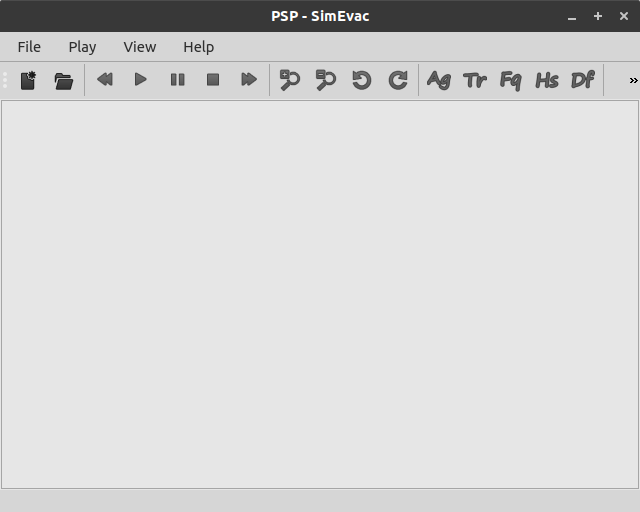
\includegraphics[width = 0.75\linewidth]{rysunki/symulator.png}
	 		\end{tightcenter}
	 		
			\caption{Główne okno symulatora.}
			\label{fig: glowne_okno_symulatora}
		\end{figure}
	
		\section{Sposób użycia}
		Do przeprowadzenia symulacji potrzebne są następujące dane wejściowe:
		\begin{itemize}
		\item plik \textit{.xml} zawierający parametry wejściowe symulacji,
		\item pliki \textit{.jpg} i \textit{.bmp} zwierające przestrzeń użytą do symulacji.
		\end{itemize}
	
		W oknie głównym programu należy wybrać opcje otwarcia pliku \textit{.xml} po czym od razu zaczyna się symulacja w czasie rzeczywistym. Po symulacji, w folderze wskazanym w pliku z parametrami zostaną wygenerowane pliki \textit{.csv} z danymi wyjściowymi symulacji.
		
		\section{Dane wejściowe i wyjściowe}
		Dane, które były wykorzystane do dalszych badań znajdowały się w:
		\begin{itemize}
		\item dane wejściowe - plik \textit{.xml},
		\item dane wyjściowe - pliki \textit{.csv}.
		\end{itemize}
		
		Danymi wejściowymi wybranymi prez autora - na podstawie łatwości modyfikacji - do dalszej analizy były:\label{dane_do_dalszej_analizy}
		
		\begin{itemize}
		\item \textbf{Panic spread factor} - współczynnik, który decyduje jak duży wpływ ma \textbf{tryb paniki} (tryb, w którym agenci zwracają mniejszą uwagę na otoczenie oraz charakteryzują się bardziej chaotycznym ruchem) na agentów.
		\item \textbf{Panic cancel zone} - współczynnik określający odległość od wyjść, w obrębie jakiej agenci mają szansę na deaktywację trybu paniki.
		\item \textbf{Cancel panic chance} - podczas testów na anulowanie trybu paniki określa procent szans na powodzenie.
		\item \textbf{Choosing evacuation path mode} - tryb wyboru drogi ewakuacyjnej przez agentów. Dostępne są 4 tryby:
			\begin{itemize}
			\item odległości,
			\item gęstości przy wyjściu,
			\item odległości oraz gęstości przy wyjściu,
			\item odległości, gęstości przy wyjściu oraz popularności wyboru wyjścia.
			\end{itemize}
		\item \textbf{Number of pedestrians} - liczba agentów biorąca udział w symulacji.
		\item \textbf{Chaos level} - szansa na aktywację trybu paniki u agentów.
		\item \textbf{Density factor} - określa wpływ współczynnika gęstości wokół agenta na funkcję kary.
		\item \textbf{Frequency factor} - określa wpływ częstości wyboru danego pola na funkcję kary.
		\item \textbf{Panic factor} - potęguje część współczynników biorących udział w obliczaniu funkcji kary. 
		\item \textbf{Distance factor} - wpływa na wybór agentów ruchu po skosie lub na wprost.
		\item \textbf{Randomness factor} - czynnik losowości dla wartości kary.
		\item \textbf{Pre-movement time mean value} oraz \textbf{Pre-movement time standard deviation} - średnia i odchylenie czasu \textit{Pre-movement}, który ma wpływ na częstotliwość wykonywania testu na zmianę obranego wyjścia przez agentów.
		\item \textbf{Speed distribution mean value} oraz \textbf{Speed distribution standard deviation} - średnia i odchylenie prędkości agentów.
		\end{itemize}
		
		Daną wyjściową wybraną do analizy był czas ewakuacji ostatniego agenta (odpowiadający czasowi ewakuacji wszystkich agentów).
		
		Dodatkowe parametry wejściowe, które były potrzebne to:
		\begin{itemize}
		\item \textbf{Repeat number} - ilość powtórzeń symulacji wykonanej na pojedynczym pliku \textit{.xml}.
		\item \textbf{Sim directory} - określa ścieżkę do folderu zawierającego pliki symulowanej przestrzeni.
		\item \textbf{Sim stat directory} - określa ścieżkę do folderu, do którego zostaną zapisane dane wyjściowe symulacji (pliki \textit{.csv}).
		\end{itemize}
		
	\chapter{Budowa modelu uczenia maszynowego}
	\textit{W tym rozdziale opisany będzie proces zbierania danych za pomocą symulatora PSP, tworzenie modelu uczenia maszynowego oraz optymalizacji jego wartości wyjściowych.}
	
		\section{Zebranie danych} \label{zebranie_danych}
		W celu zebrania danych, które miałyby trafić później do modelu uczenia maszynowego, został stworzony skrypt pythonowy, który wygenerował 200 różnych zestawów parametrów wejściowych do symulatora. Rodzaje danych, które zostały wygenerowane znajdują się w rozdziale~\ref{dane_do_dalszej_analizy}. Dla każdego zestawu danych autor ustawił parametr \textit{Repeat number} na wartość \textbf{10}, dzięki czemu dla każdego zestawu danych wejściowych generowane było 10 zestawów danych wyjściowych. Było to niezwykle cenne z 2 powodów:
		\begin{itemize}
		\item Do symulatora trzeba było ręcznie ładować plik \textit{.xml}, a dzięki temu z jedngo pliku otrzymywałem od razu 10 zestawów plików wyjściowych.
		\item Ruchy agentów, z takim samym zestawem parametrów, rożnią się między symulacjami, a dzięki powtórzeniom można było łatwiej odczytać ich trend.
		\end{itemize}
		
		Symulowaną przestrzenią był bydunek należący do kompleksu AGH - Centrum Dydaktyki U2. Jest ona widoczna na rysunku~\ref{fig: agh_u2_centrum_dydaktyki}.
		
		\begin{figure}[h]
			\begin{tightcenter}
			 	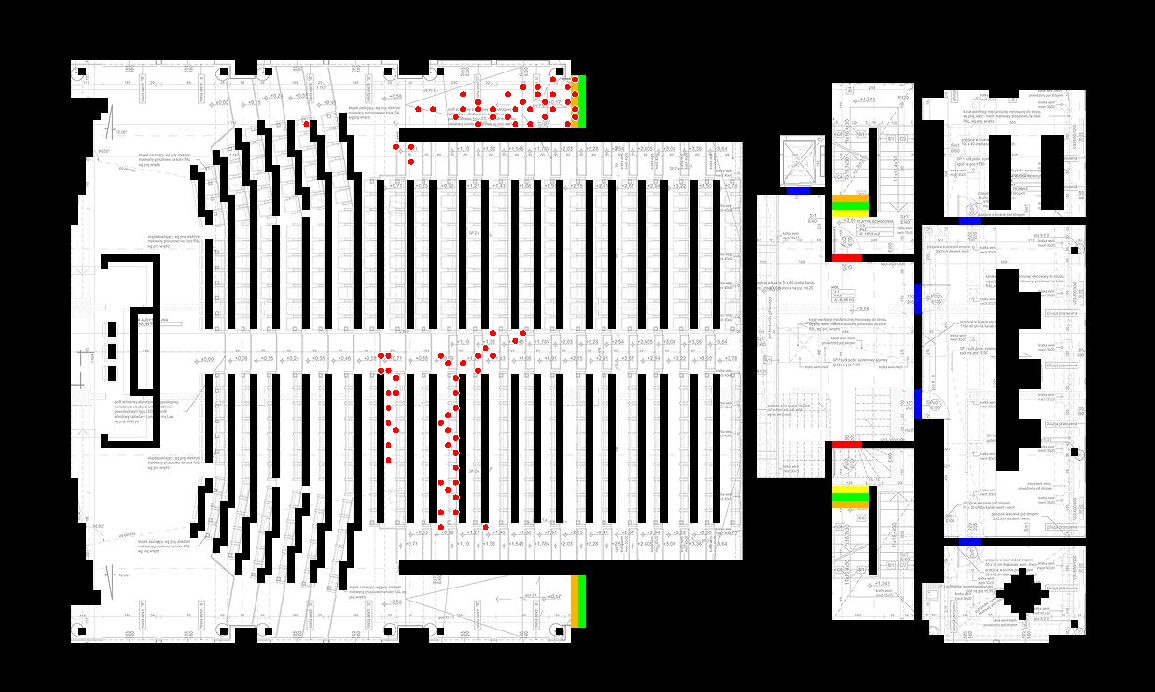
\includegraphics[width = \linewidth]{rysunki/agh_u2.png}
			\end{tightcenter}	 			
			 			
		 	\caption{Widok przestrzeni AGH U2 Centrum Dydaktyki w symulatorze PSP.}
			\label{fig: agh_u2_centrum_dydaktyki}
		\end{figure}
		
		Każdy zestaw danych zawierał \textbf{15} parametrów wejściowych oraz \textbf{1} parametr wyjściowy. Z tak przygotowanymi danymi autor miał możliwość stworzenia pierwszego modelu.
		
		\section{Pierwszy model - tworzenie i analiza} \label{pierwszy_model_tworzenie_i_analiza}
		Dla powyższych zastosowań swtorzony został model \textit{Perceptron} posiadający pojedyncze wyjście oraz nie posiadający funkcji aktywacji - jako że model miał służyć do regresji a nie klasyfikacji. Zestawy danych zostały podzielone w stosunku 80\% : 20\% na \textbf{dane treningowe} i \textbf{dane testowe}, pozwala to na trenowanie sieci na danych treningowych oraz sprawdzanie jej efektywności na danych testowych co daje możliwość walidacji tego, jak dobrze sieć radzi sobie z danymi, z którymi nie miała styczności.
		
		Podsumowując, parametry pierwszego modelu były następujące:
		\begin{itemize}
		\item pojedyncza warstwa składająca się z jednego neuronu,
		\item \textbf{funkcja aktywacji} - brak,
		\item \textbf{współczynnik uczący} - 0.1,
		\item \textbf{metryka do optymalizacji} - \textit{MSE},
		\item \textbf{liczba epok uczacych} - 300,
		\item podział na \textbf{dane treningowe} i \textbf{dane testowe} - 80\% : 20\%.
		\end{itemize}
				
		Proces uczący został wykonany 10 razy od nowa na nienauczonym modelu, za kazdym razem wykonując permutację danych. Średnie \textit{MSE} danych wyglądają następująco:
		\begin{itemize}
		\item \textbf{średni MSE danych treningowych} - 147,77 ($\pm$16,04),
		\item \textbf{średni MSE danych testowych} - 166,18 ($\pm$50,77).
		\end{itemize}
		Wykres zależności \textit{MSE} danych od iteracji uczacej najlepszego przypadku (biorąc pod uwagę \textit{MSE} danych testowych) jest widoczna na rysunku \ref{fig: pierwszy_model_wykres_uczenia}. Taki rodzaj wykresów będzie nazywany dalej \textbf{wykresami krzywych uczących dla najlepszego przypadku}. Analizując go, autor doszedł do następujących wniosków:
		\begin{itemize}
		\item \textit{MSE} danych treningowych jak i testowych jest na wysokim poziomie co oznacza, że model ma \textbf{wysoki bias}. Oznacza to, że użyty model jest zbyt prosty i nie ważne jak dużo danych zostanie do niego podanych i jak długo będzie się on uczył - \textit{MSE} danych nie obniży się poniżej pewnego poziomu.
		\item Podczas uczenia \textit{MSE} danych jest obarczony dużym szumem, co oznacza niestabilność danych lub modelu.
		\item \textit{MSE} danych testowych jest przez większość iteracji mniejsze niż treningowych co oznacza, że dla danych których sieć nie widziała, przewiduje ona wartości bliższe prawdzie niż na danych na których się uczyła. Jest to niecodzienne zachowanie co również dowodzi niestabilności modelu lub danych.
		\end{itemize}
		
		\begin{figure}[h]
	 		\begin{tightcenter}
	 			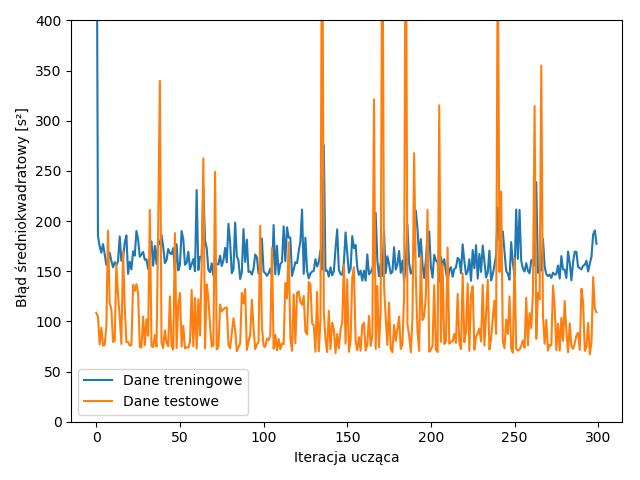
\includegraphics[width = \linewidth]{wykresy/1_pierwszy_model_tworzenie_i_analiza/wykres_uczenia.png}
	 		\end{tightcenter}
	 		
 			\caption{Krzywe uczące dla najlepszego przypadku w pierwszym modelu.}
			\label{fig: pierwszy_model_wykres_uczenia}
		\end{figure}
		
		W celu zbadania tego, jaki wpływ ma ilość danych na których się uczy sieć na \textit{MSE} tych danych - autor postanowił uruchomić proces uczący kolejne 20 razy dla pojedynczej permutacji danych wejściowych, lecz przy zwiększającej się ilości danych treningowych. Przykładowy wykres obrazujący wynik tych badań jest widoczny na rysunku \ref{fig: pierwszy_model_learning_curves}. Ten rodzaj wykresów dalej nazywany będzie \textbf{wykresami krzywych uczących dla zmiennej ilości danych}. Informacją jaką można z niego odczytać jest ilość danych potrzebna do tego, aby osiągnąć dany pułap \textit{MSE} danych. Widać, że większa ilość danych nie spowodowała spadku \textit{MSE} danych treningowych ani danych testowych.
		
		\begin{figure}[h]
	 		\begin{tightcenter}
	 			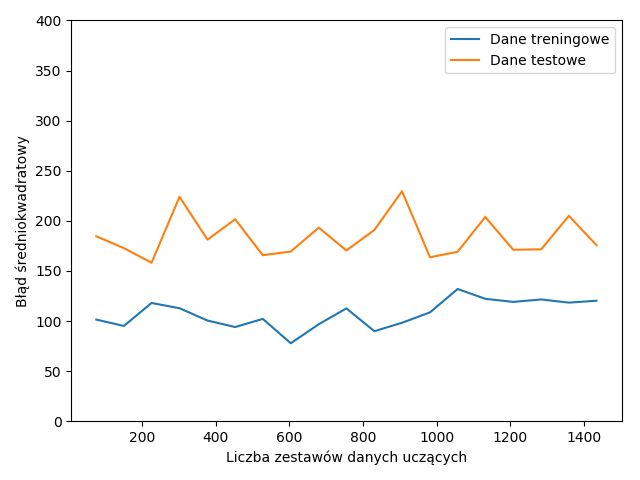
\includegraphics[width = \linewidth]{wykresy/1_pierwszy_model_tworzenie_i_analiza/learning_curves.png}
	 		\end{tightcenter}
	 		
 			\caption{Krzywe uczące dla zmiennej ilości danych w pierwszym modelu.}
			\label{fig: pierwszy_model_learning_curves}
		\end{figure}
		
		Podsumowując, obecny model ma wysoki bias - jest zbyt prosty dla danych, przez co większa ich ilość oraz dłuższy proces uczący nie dają żadnych efektów. Na wykresach widać niestabilność modelu lub danych, co powoduje bardzo duże szumy na wykresach \textit{MSE}. Co więcej - niepokojący jest fakt, że \textit{MSE} danych testowych był często niższy niż \textit{MSE} danych treningowych.
		
		\section{Normalizacja danych} \label{normalizacja_danych}
		Mając na uwadze problemy stworzonego modelu, w pierwszej kolejności autor postanowił przejrzeć dane wejściowe do modelu. Ze wszystkich zestawów danych obliczona została średnia każdego z parametrów wejściowych do sieci neuronowej. Wyniki są widoczne w tabeli \ref{porownanie_srednich_wartosci_i_odchylen_parametrow_wejsciowych_modelu}. Widać w niej, że niektóre parametry mają wartości 2 rzędy wielkości większe niż inne. Takie różnice pomiędzy różnymi parametrami wejściowymi powodują faworyzowanie przez sieć jednych parametrów ponad drugie. Autor postanowił więc zastosować normalizację danych według wzoru:
		
		\begin{equation}
		X_{new} = \frac{X_{old} - \mu}{\sigma}
		\end{equation}		 
		
		Gdzie:
		\begin{itemize}
		\item $\mu$ - wektor średniej parametrów,
		\item $\sigma$ - wektor odchylenia standardowego parametrów.
		\end{itemize}
		
		\begin{table}[t]
			\caption{Porównanie średnich wartości parametrów wejściowych do modelu.}
			\begin{mytabular}{r c}
					\multicolumn{1}{c}{Nazwa parametru} & Średnia wartość \\
					Panic spread factor & 1.74 \\
					Panic cancel zone & 0.53 \\
					Cancel panic chance& 51.59 \\
					Choosing evacuation path mode & 2.53 \\
					Number of pederastian& 271.8 \\
					Chaos level & 53.9 \\
					Density factor & 5.26 \\
					Frequency factor & 5.33 \\
					Panic factor & 1.45 \\
					Distance factor & 2.51 \\
					Randomness factor & 0.49 \\
					Pre-movement time mean value & 5.44 \\
					Pre-movement time standard deviation & 0.51 \\
					Speed distribution mean value & 5.62 \\
					Speed distribution standard deviation & 0.54
			\end{mytabular}
			\label{porownanie_srednich_wartosci_i_odchylen_parametrow_wejsciowych_modelu}
		\end{table}
		
		Posiadając tak przygotowane dane zostały wykonane - tak jak w punkcie \ref{pierwszy_model_tworzenie_i_analiza} - 10 cykli nauczania z różnymi permutacjami danych oraz 20 cykli z jedną permutacją, lecz zmieniającym się rozmiarem zestawu danych treningowych. Średnie \textit{MSE} danych są następujące:
		\begin{itemize}
		\item \textbf{średni MSE danych treningowych} - 118,64 ($\pm$6,07),
		\item \textbf{średni MSE danych testowych} - 130,70 ($\pm$23,47).
		\end{itemize}
		Wykres krzywych uczących dla najlepszego przypadku widoczny jest na rysunku \ref{fig: pierwszy_model_wykres_uczenia_z_normalizacja}. Dodatkowo patrząc na wykres krzywych uczących dla zmiennej ilości danych z rysunku \ref{fig: pierwszy_model_learning_curves_z_normalizacja} - widać zależność \textit{MSE} danych od liczby danych treningowych. 
		
		\begin{figure}[h]
			\begin{tightcenter}
	 			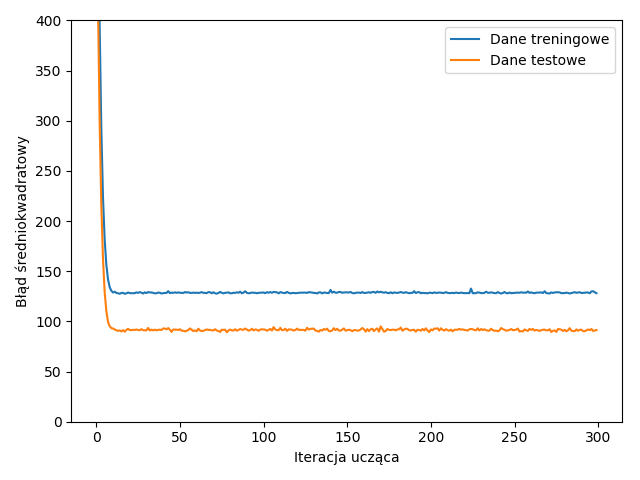
\includegraphics[width = \linewidth]{wykresy/2_normalizacja_danych/wykres_uczenia.png}
	 		\end{tightcenter}
	 		
 			\caption{Krzywe uczące dla najlepszego przypadku w pierwszym modelu ze znormalizowanymi danymi.}
			\label{fig: pierwszy_model_wykres_uczenia_z_normalizacja}
		\end{figure}
		
		\begin{figure}[h]
			\begin{tightcenter}
	 			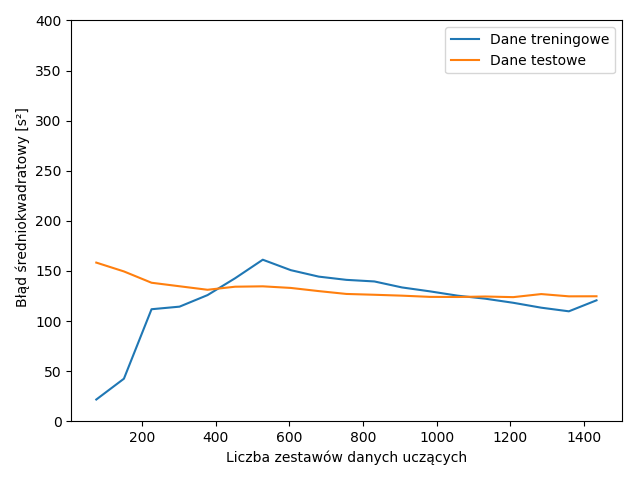
\includegraphics[width = 0.75\linewidth]{wykresy/2_normalizacja_danych/learning_curves.png}
	 		\end{tightcenter}
	 		
 			\caption{Krzywe uczące dla zmniennej ilości danych w pierwszym modelu ze znormalizowanymi danymi.}
			\label{fig: pierwszy_model_learning_curves_z_normalizacja}
		\end{figure}
		
		Podsumowując, pierwszą rzeczą rzucającą się w oczy jest duża stabilność wartości na wykresach - eliminuje to sytuacje w których wynik uczenia był winą przypadku, jako że kilka iteracji wcześniej lub później \textit{Perceptron} dawał zupełnie inny rezultat. Dzięki większej stabilności sieci łatwiej jest także wyciągać wnioski na podstawie wykresów. Lepiej widoczny jest problem zauważony wcześniej - wysoki bias modelu. Objawia się on tym, że na początku \textit{MSE} danych maleje, aż do pewnego momentu gdzie jest stały i żadna ilość danych albo długość uczenia nie spowoduje jego zmniejszenia. Ostatnią rzeczą, która jest taka sama jak w rozdziale \ref{pierwszy_model_tworzenie_i_analiza} - \textit{MSE} danych testowych często jest mniejsze niż danych treningowych.
		
		\section{Drugi model - tworzenie i analiza} \label{drugi_model_tworzenie_i_analiza}
		Chcąc rozwiązać główny problem poprzedniego modelu - wysoki bias - autor potrzebował modelu, który potrafi nauczyć się bardziej skomplikowanych funkcji. Takim modelem była sieć neuronowa z kilkoma warstwami. Dzięki każdej następnej warstwie ma ona możliwość uczenia się coraz bardziej skomplikowanych funkcji. Stworzona sieć miała 1 \textbf{warstwę ukrytą} - warstwę neuronów pomiędzy wejściami a warstwą wyjść - z 30 neuronami. Jako funkcję aktywacji wybrałem funkcję \textit{ReLU}.
		Podsumowując, parametry drugiego modelu były następujące:
		\begin{itemize}
			\item 1 warstwa ukryta z 30 neuronami i funkcją aktywacji \textit{ReLU},
			\item warstwa wyjściowa składająca się z jednego neuronu bez funkcji aktywacji,
			\item \textbf{współczynnik uczący} - 0.1,
			\item \textbf{metryka do optymalizacji} - MSE,
			\item \textbf{liczba epok uczacych} - 300,
			\item podział na \textbf{dane treningowe} i \textbf{dane testowe} - 80\% : 20\%.
		\end{itemize}
		
		Proces uczący przeprowadzony został identycznie jak poprzednio - autor wykonał 10 osobnych cykli uczących z różnymi permutacjami danych oraz 20 osobnych cykli uczących na zmieniającej się wielkości zestawu danych traningowych. Średnie \textit{MSE} danych z 10 cykli są następujące:
		\begin{itemize}
		\item \textbf{średni MSE danych treningowych} - 47,47 ($\pm$6,08),
		\item \textbf{średni MSE danych testowych} - 73,66 ($\pm$25,77).
		\end{itemize}
		Wykres krzywych uczacych dla najlepszego przypadku widoczny jest na rysunku \ref{fig: drugi_model_wykres_uczenia} a krzywych uczących dla zmiennej ilości danych - na rysunku \ref{fig: drugi_model_learning_curves}.
		
		\begin{figure}[h]
			\begin{tightcenter}
	 			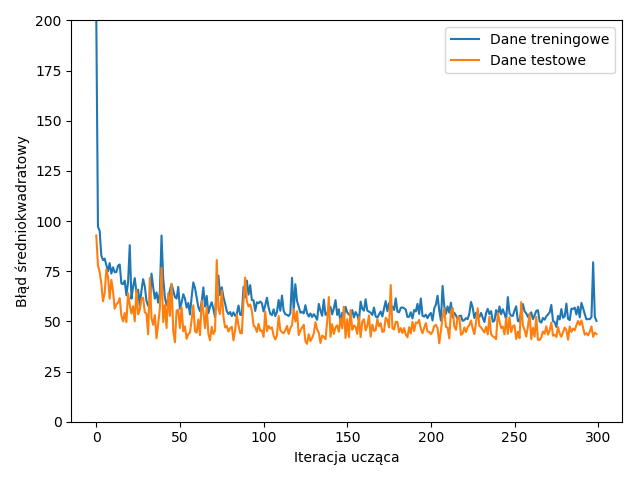
\includegraphics[width = \linewidth]{wykresy/3_drugi_model_tworzenie_i_analiza/wykres_uczenia.png}
	 		\end{tightcenter}
	 		
 			\caption{Krzywe uczące dla najlepszego przypadku w drugim modelu.}
			\label{fig: drugi_model_wykres_uczenia}
		\end{figure}
		
		\begin{figure}[h]
			\begin{tightcenter}
	 			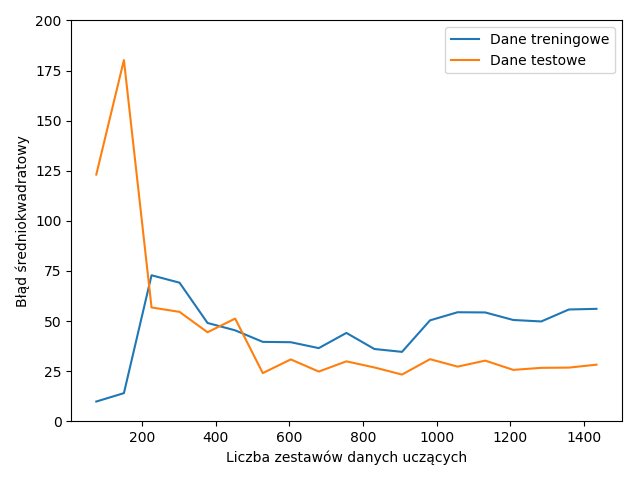
\includegraphics[width = \linewidth]{wykresy/3_drugi_model_tworzenie_i_analiza/learning_curves.png}
	 		\end{tightcenter}
	 		
 			\caption{Krzywe uczące dla zmiennej ilości danych w drugim modelu.}
			\label{fig: drugi_model_learning_curves}
		\end{figure}
		
		Porównując te dane z tymi z sekcji \ref{normalizacja_danych} widać znaczącą poprawę modelu - trzykrotny spadek średnich \textit{MSE} danych treningowych oraz testowych. Mimo tego widać, \textit{MSE} po osiągnięciu pewnego pułapu przestaje maleć - oznacza to, że model dalej ma duży bias.
		
		\section{Zwiększenie stopnia skomplikowania modelu} \label{zwiekszenie_stopnia_skomplikowania_modelu}
		Próbując zmniejszyć bias sieci neuronowej, autor postanowił przeprowadzić eksperymenty z innymi parametrami sieci, a mianowicie:
		\begin{itemize}
		\item liczba warstw ukrytych - \textbf{1}, liczba neuronów w warstwie - \textbf{40};
		\item liczba warstw ukrytych - \textbf{2}, liczba neuronów w każdej warstwie - \textbf{20};
		\item liczba warstw ukrytych - \textbf{2}, liczba neuronów w każdej warstwie - \textbf{40};
		\end{itemize}
		
		Zestawienie wynikow z sekcji \ref{drugi_model_tworzenie_i_analiza} oraz powyższych kombinacji parametrów jest następujące:
		\begin{itemize}
		\item krzywe uczące dla najlepszych przypadków są widoczne na rysunku \ref{fig: drugi_model_kombinacje_parametrow_wykresy_uczenia},
		\item krzywe uczące dla zmiennej ilości danych pokazane są na rysunku \ref{fig: drugi_model_kombinacje_parametrow_learning_curves}.
		\end{itemize}
		
		Dodatkowo średnie \textit{MSE} z 10 różnych permutacji danych zostały zestawione w tabeli \ref{porownanie_srednich_wartosci_mse_dla_roznych_kombinacji_parametrow_sieci}.
		
		\begin{table}[t]
			\caption{Porównanie średnich wartości \textit{MSE} danych dla różnych kombinacji parametrów sieci.}
			\begin{mytabular}{c L L L}
					Ilość warstw & Ilość neuronów w warstwie & MSE danych treningowych & MSE danych testowych \\
					1 & 20 & 47,47 ($\pm$6,08) & 73,66 ($\pm$25,77) \\
					1 & 40 & 53,16 ($\pm$4,93) & 47,87 ($\pm$20,13) \\
					2 & 20 & 59,49 ($\pm$10,81) & 89,52 ($\pm$22,04) \\
					2 & 40 & 64,13 ($\pm$7,30) & 70,68 ($\pm$20,42)
			\end{mytabular}
			\label{porownanie_srednich_wartosci_mse_dla_roznych_kombinacji_parametrow_sieci}
		\end{table}

		\begin{figure}[h]
			\begin{subfigure}{.5\linewidth}
		 		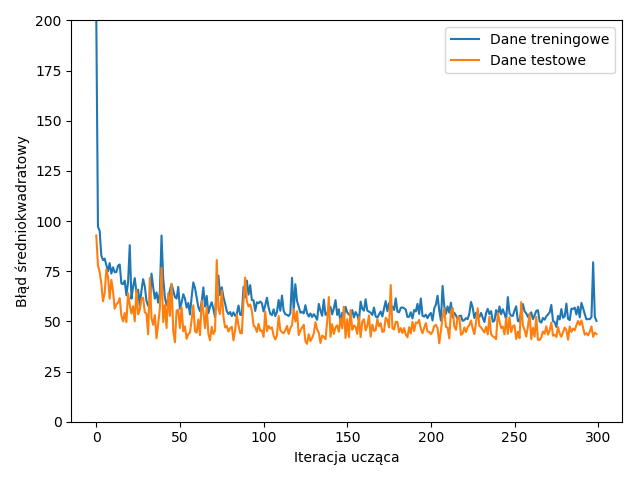
\includegraphics[width =\linewidth]{wykresy/3_drugi_model_tworzenie_i_analiza/wykres_uczenia.png}
		 		\caption{1 warstwa ukryta, 20 neuronow w każdej warstwie}
		 	\end{subfigure}
		 	\begin{subfigure}{.5\linewidth}
		 		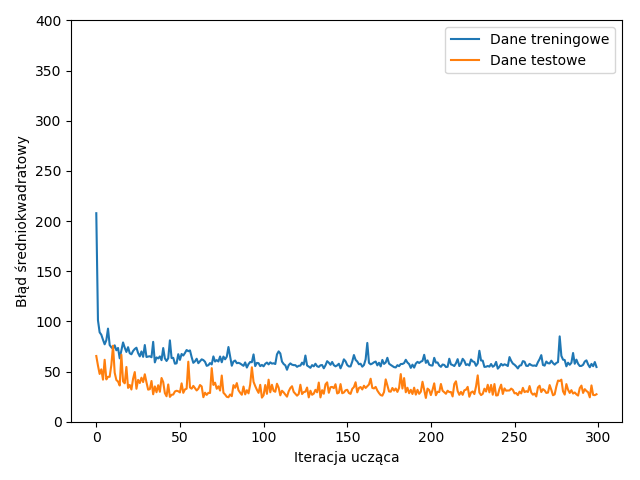
\includegraphics[width =\linewidth]{wykresy/4_zwiekszenie_stopnia_skomplikowania_modelu/1_warstwa_40_neuronow_wykres_uczenia.png}
		 		\caption{1 warstwa ukryta, 40 neuronow w każdej warstwie}
		 	\end{subfigure}
		 	
		 	\begin{subfigure}{.5\linewidth}
		 		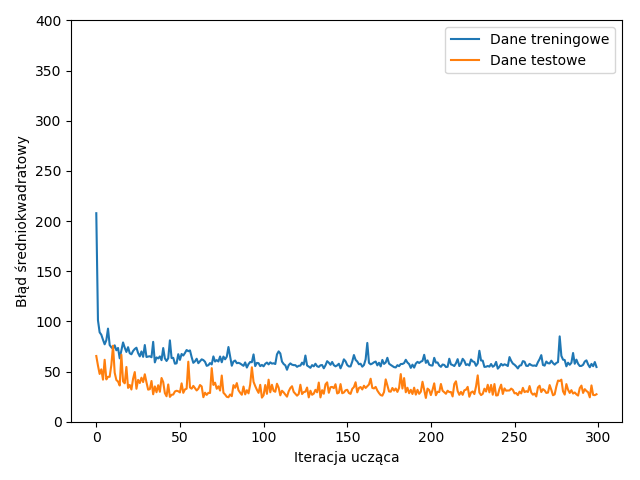
\includegraphics[width =\linewidth]{wykresy/4_zwiekszenie_stopnia_skomplikowania_modelu/2_warstwy_20_neuronow_wykres_uczenia.png}
		 		\caption{2 warstwy ukryte, 20 neuronow w każdej warstwie}
		 	\end{subfigure}
		 	\begin{subfigure}{.5\linewidth}
		 		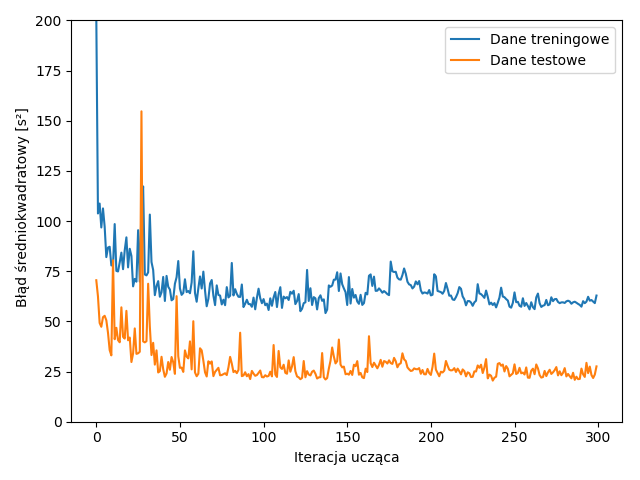
\includegraphics[width =\linewidth]{wykresy/4_zwiekszenie_stopnia_skomplikowania_modelu/2_warstwy_40_neuronow_wykres_uczenia.png}
		 		\caption{2 warstwy ukryte, 40 neuronow w każdej warstwie}
		 	\end{subfigure}
	 	
 			\caption{Krzywe uczące dla najlepszych przypadków przy użyciu różnych kombinacji parametrów w drugim modelu.}
			\label{fig: drugi_model_kombinacje_parametrow_wykresy_uczenia}
		\end{figure}
		
		\begin{figure}[h]
			\begin{subfigure}{.5\linewidth}
		 		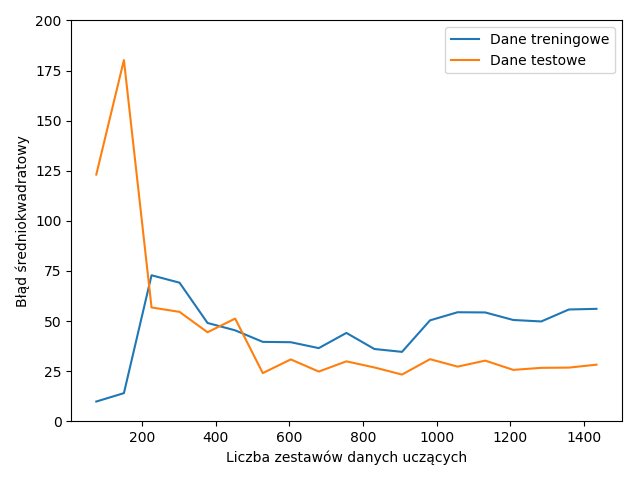
\includegraphics[width =\linewidth]{wykresy/3_drugi_model_tworzenie_i_analiza/learning_curves.png}
		 		\caption{1 warstwa ukryta, 20 neuronow w każdej warstwie}
		 	\end{subfigure}
		 	\begin{subfigure}{.5\linewidth}
		 		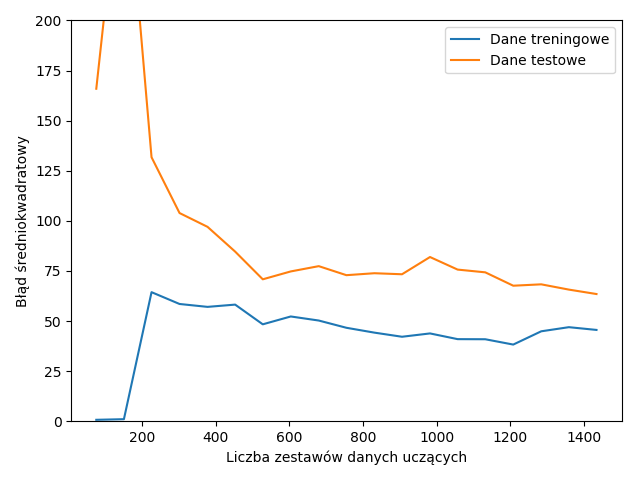
\includegraphics[width =\linewidth]{wykresy/4_zwiekszenie_stopnia_skomplikowania_modelu/1_warstwa_40_neuronow_learning_curves.png}
		 		\caption{1 warstwa ukryta, 40 neuronow w każdej warstwie}
		 	\end{subfigure}
		 	
		 	\begin{subfigure}{.5\linewidth}
		 		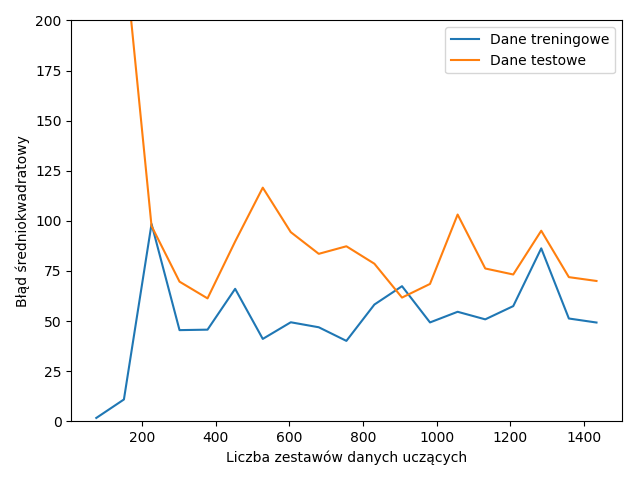
\includegraphics[width =\linewidth]{wykresy/4_zwiekszenie_stopnia_skomplikowania_modelu/2_warstwy_20_neuronow_learning_curves.png}
		 		\caption{2 warstwy ukryte, 20 neuronow w każdej warstwie}
		 	\end{subfigure}
		 	\begin{subfigure}{.5\linewidth}
		 		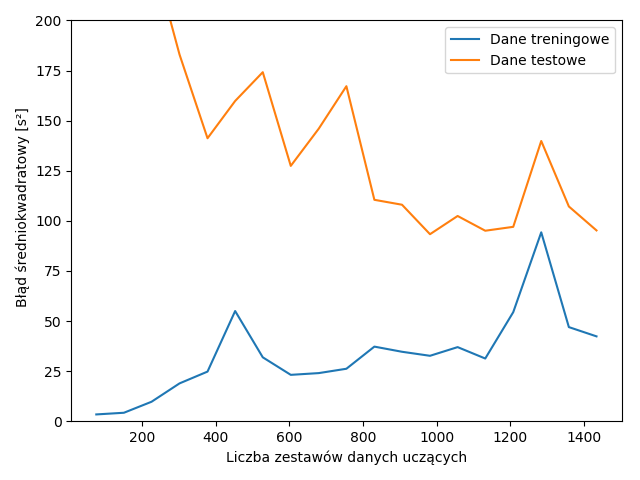
\includegraphics[width =\linewidth]{wykresy/4_zwiekszenie_stopnia_skomplikowania_modelu/2_warstwy_40_neuronow_learning_curves.png}
		 		\caption{2 warstwy ukryte, 40 neuronow w każdej warstwie}
		 	\end{subfigure}
	 	
 			\caption{Krzywe uczące dla zmiennej ilosci danych przy różnych kombinacjach parametrów w drugim modelu.}
			\label{fig: drugi_model_kombinacje_parametrow_learning_curves}
		\end{figure}
		
		Mimo zwiększenia stopnia skomplikowania sieci, \textit{MSE} danych treningowych i testowych nie wykazywały tendencji spadkowej. To co powinno się stać w takim przypadku, to \textit{MSE} danych treningowych powinien osiągać coraz niższe wartości wraz ze skomplikowaniem modelu. Na wykresach również widac, że dane testowe miały czasem \textit{MSE} mniejszych od zestawu treningowego. Wnioskiem tej analizy jest to, że problem z uczeniem sieci leży nie w modelu, a w danych.
		
		\section{Uśrednianie danych} \label{usrednianie_danych}
		Wiedząc że problem leży w danych autor postanowił ulepszyć istniejące dane, uśredniając je. W sekcji \ref{zebranie_danych} autor napisał, że dla każdego zbioru parametrów wejściowych wygenerowane zostało 10 zbiorów parametrów wyjściowych. Dla każdego zestawu wejściowego obliczona została średnia zestawów parametrów wyjściowych co zmniejszyło ilość danych 10-krotnie. Ostatecznie nowy zbiór zawierał 200 zestawów danych (przy czym, podczas procesu uczenia zostały one podzielone na dane treningowe i testowe).
		
		Po przetworzeniu danych autor postanowił powtórzyć badanie z sekcji \ref{zwiekszenie_stopnia_skomplikowania_modelu}, używając kombinacji parametrów:
		\begin{itemize}
		\item ilość warstw ukrytych - \textbf{1} i \textbf{2},
		\item ilość neuronów w każdej warstwie - \textbf{20} i \textbf{40}.
		\end{itemize}
		
		Po powtórzeniu poprzedniego badania na uśrednionych danych, wyniki widać na rysunkach \ref{fig: drugi_model_przy_usrednionych_danych_wykresy_uczenia} i \ref{fig: drugi_model_przy_usrednionych_danych_learning_curves}. Średnie \textit{MSE} danych dla kombinacji parametrów jest umieszczone w tabeli \ref{porownanie_srednich_wartosci_mse_przy_usrednionych_danych}. 

		\begin{table}[t]
			\caption{Porównanie średnich wartości \textit{MSE} danych przy uśrednionych danych.}
			\begin{mytabular}{c L L c}
					Ilość warstw & Ilość neuronów w warstwie & MSE danych treningowych & MSE danych testowych \\
					1 & 20 & 1,38 ($\pm$0,81) & 189,06 ($\pm$60,12) \\
					1 & 40 & 2,21 ($\pm$2,02) & 182,91 ($\pm$50,58) \\
					2 & 20 & 6,06 ($\pm$8,93) & 113,56 ($\pm$55,77) \\
					2 & 40 & 2,02 ($\pm$4,38) & 108,03 ($\pm$40,39)
			\end{mytabular}
			\label{porownanie_srednich_wartosci_mse_przy_usrednionych_danych}
		\end{table}

		\begin{figure}[h]
			\begin{subfigure}{.5\linewidth}
		 		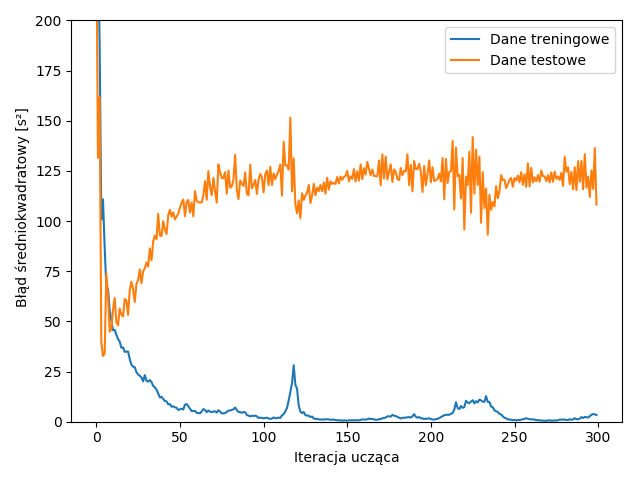
\includegraphics[width =\linewidth]{wykresy/5_usrednianie_danych/1_warstwa_20_neuronow_wykres_uczenia.png}
		 		\caption{1 warstwa ukryta, 20 neuronow w każdej warstwie}
		 	\end{subfigure}
		 	\begin{subfigure}{.5\linewidth}
		 		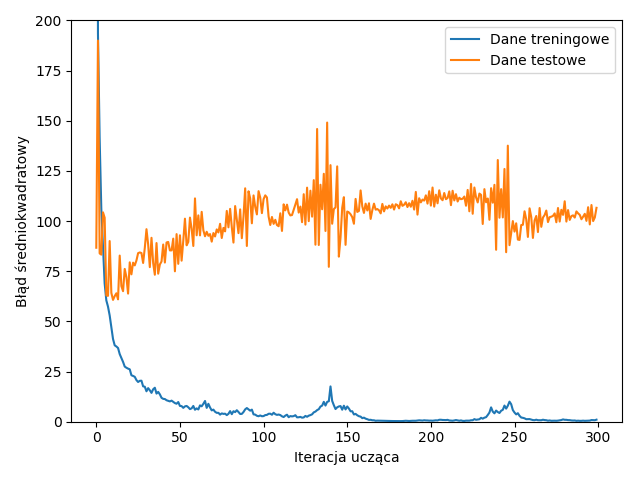
\includegraphics[width =\linewidth]{wykresy/5_usrednianie_danych/1_warstwa_40_neuronow_wykres_uczenia.png}
		 		\caption{1 warstwa ukryta, 40 neuronow w każdej warstwie}
		 	\end{subfigure}
		 	
		 	\begin{subfigure}{.5\linewidth}
		 		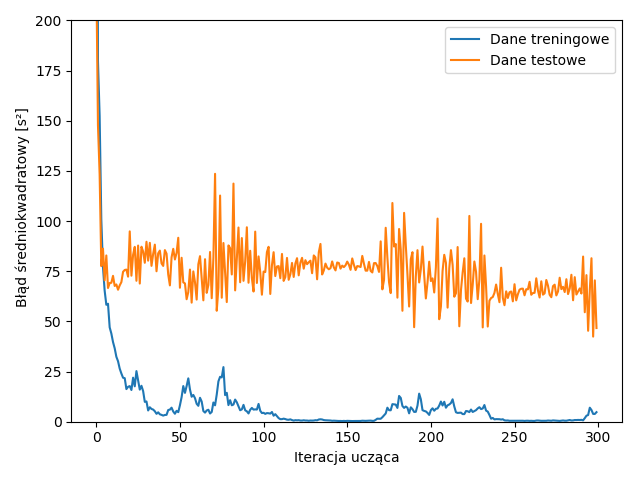
\includegraphics[width =\linewidth]{wykresy/5_usrednianie_danych/2_warstwy_20_neuronow_wykres_uczenia.png}
		 		\caption{2 warstwy ukryte, 20 neuronow w każdej warstwie}
		 	\end{subfigure}
		 	\begin{subfigure}{.5\linewidth}
		 		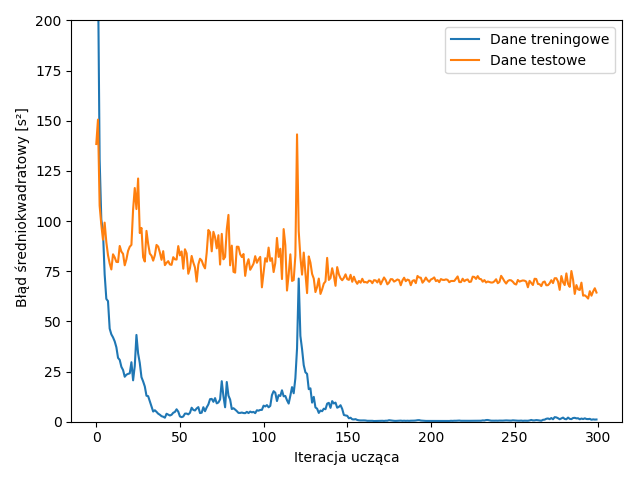
\includegraphics[width =\linewidth]{wykresy/5_usrednianie_danych/2_warstwy_40_neuronow_wykres_uczenia.png}
		 		\caption{2 warstwy ukryte, 40 neuronow w każdej warstwie}
		 	\end{subfigure}
	 	
 			\caption{Krzywe uczące dla najlepszych przypadków przy uśrednionych danych w drugim modelu.}
			\label{fig: drugi_model_przy_usrednionych_danych_wykresy_uczenia}
		\end{figure}
		
		\begin{figure}[h]
			\begin{subfigure}{.5\linewidth}
		 		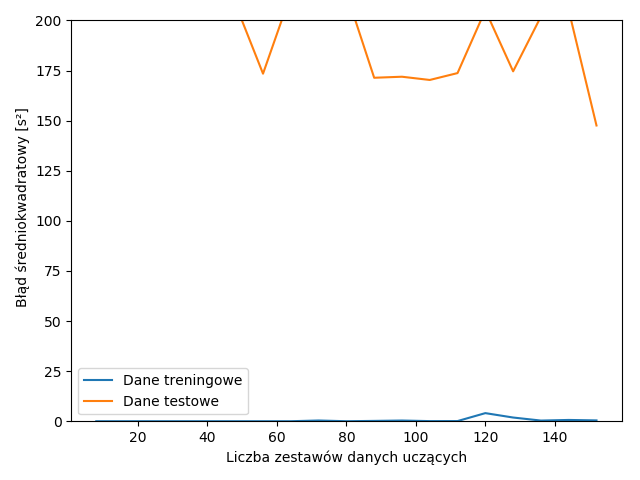
\includegraphics[width =\linewidth]{wykresy/5_usrednianie_danych/1_warstwa_20_neuronow_learning_curves.png}
		 		\caption{1 warstwa ukryta, 20 neuronow w każdej warstwie}
		 	\end{subfigure}
		 	\begin{subfigure}{.5\linewidth}
		 		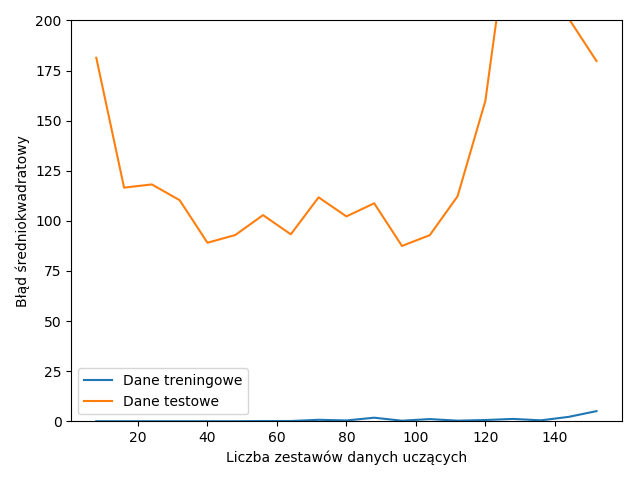
\includegraphics[width =\linewidth]{wykresy/5_usrednianie_danych/1_warstwa_40_neuronow_learning_curves.png}
		 		\caption{1 warstwa ukryta, 40 neuronow w każdej warstwie}
		 	\end{subfigure}
		 	
		 	\begin{subfigure}{.5\linewidth}
		 		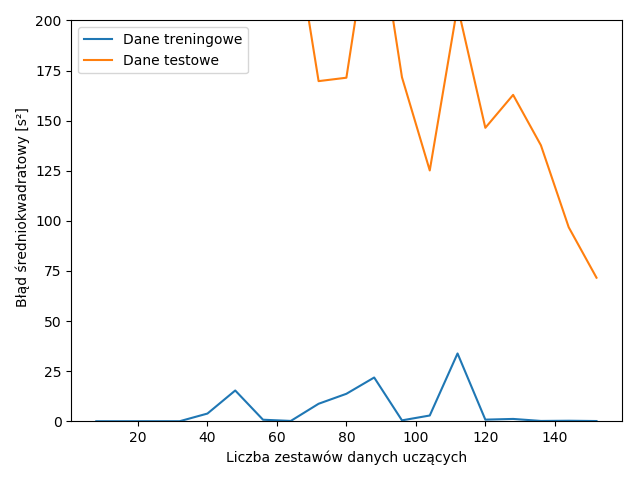
\includegraphics[width =\linewidth]{wykresy/5_usrednianie_danych/2_warstwy_20_neuronow_learning_curves.png}
		 		\caption{2 warstwy ukryte, 20 neuronow w każdej warstwie}
		 	\end{subfigure}
		 	\begin{subfigure}{.5\linewidth}
		 		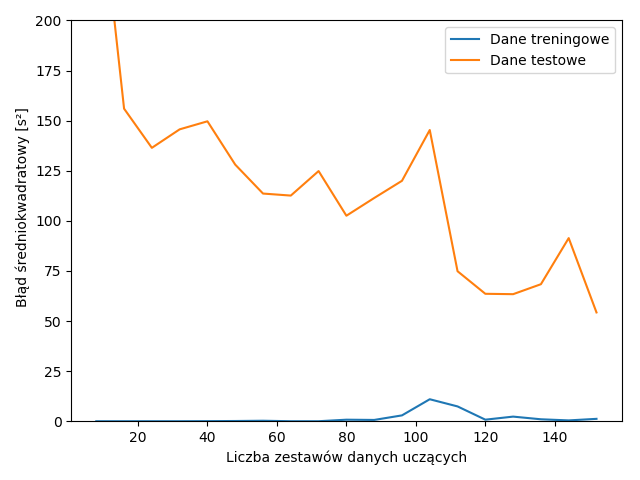
\includegraphics[width =\linewidth]{wykresy/5_usrednianie_danych/2_warstwy_40_neuronow_learning_curves.png}
		 		\caption{2 warstwy ukryte, 40 neuronow w każdej warstwie}
		 	\end{subfigure}
	 	
 			\caption{Krzywe uczące dla zmniennej ilości uśrednionych danych w drugim modelu.}
			\label{fig: drugi_model_przy_usrednionych_danych_learning_curves}
		\end{figure}
		
		Analizując dane, można zauważyć że po uśrednieniu zachowują się one zgodnie z przewidywaniami - większe skomplikowanie sieci neuronowej zmniejszyło dramatycznie \textit{MSE} danych treningowych. Co było również spodziewane - \textit{MSE} danych testowych pozostał wysoki; jednakże na wykresach \ref{fig: drugi_model_przy_usrednionych_danych_learning_curves} (c) i (d) widać ciekawą tendencję - wygląda na to, że przy większych rozmiarach zbioru danych nawet \textit{MSE} zbioru testowego zaczyna się obniżać. Podobną tendencję, lecz słabszą można też zauwazyć na wykresach \ref{fig: drugi_model_przy_usrednionych_danych_learning_curves} (a) i (b) po przekroczeniu pułapu 140 zestawów danych uczących. Gdy model jest zbyt dobrze przyuczony do danych treningowych i źle generalizuje na danych testowych, mówi się że posiada on \textbf{wysoką wariancję}.
		
		\section{Regularyzacja modelu} \label{regularyzacja_modelu}
		Chcąc obnizyć wariancję modelu uczenia maszynowego stosuje się techniki zwane regularyzacją. Najprostsze z nich czyli regularyzacja \textbf{L1} i \textbf{L2} polegają na dodaniu współczynnika kary do funkcji kosztu. Karze ona model za posiadanie wysokich wag na połączeniach pomiędzy neuronami. Dla porównania mając funkcję kosztu \ref{loss_function}, używając regularyzacji \textit{L1} będzie ona wyglądać jak na równaniu \ref{loss_function_l1} a regularyzacji \textit{L2} - tak jak na równaniu \ref{loss_function_l2}. Współczynnik $\lambda$ to tak zwany \textbf{współczynnik regularyzacji} - odpowiada on za siłę, z jaką wagi będa zmniejszane.
		
		\begin{equation} \label{loss_function}
		S = \sum_{i = 1}^n (y_i - f(x_i))^2
		\end{equation}
		\begin{equation} \label{loss_function_l1}
		S = \sum_{i = 1}^n (y_i - f(x_i))^2 + \lambda \sum_{i = 1}^k |w_i|
		\end{equation}
		\begin{equation} \label{loss_function_l2}
		S = \sum_{i = 1}^n (y_i - f(x_i))^2 + \lambda \sum_{i = 1}^k w_i^2
		\end{equation}
		
		Bazując na badaniach z poprzedniego rozdziału, autor wybrał model z jedną 20-neuronową warstwą ukrytą aby przeprowadzić na nim eksperymenty z regularyzacją. Wybór był umotywowany tym, że był to najprostszy z 4 modeli, a jednocześnie miał możliwość prawie idealnego nauczenia się danych treningowych. Wybrane do badań parametry regularyzacji to:
		\begin{itemize}
		\item funkcje regularyzujące - \textbf{L1} i \textbf{L2},
		\item parametr regularyzacji $\lambda$ - \textbf{0,1}; \textbf{0,3}; \textbf{1}; \textbf{3}.
		\end{itemize}
		
		Po przeprowadzeniu eksperymentów ze wszystkimi powyższymi kombinacjami parametrów wyrysowane zostały wykresy krzywych uczących dla najlepszych przypadków na rysunkach \ref{fig: drugi_model_przy_regularyzacji_l1_wykresy_uczenia} i \ref{fig: drugi_model_przy_regularyzacji_l2_wykresy_uczenia} oraz wykresy krzywych uczących dla zmiennej ilości danych na rysunkach \ref{fig: drugi_model_przy_regularyzacji_l1_learning_curves} i \ref{fig: drugi_model_przy_regularyzacji_l2_learning_curves}. Dodatkowo zestawienie średnich \textit{MSE} dla owych kombinacji umieściłem w tabeli \ref{porownanie_srednich_wartosci_mse_przy_regularyzacji}.
		
		\begin{table}[t]
			\caption{Porównanie średnich wartości \textit{MSE} danych przy regularyzacji.}
			\begin{mytabular}{L L L c}
					Rodzaj regularyzacji & Ilość neuronów w warstwie & MSE danych treningowych & MSE danych testowych \\
					L1 & 0,1 & 11,65 ($\pm$15,70) & 99,61 ($\pm$43,27) \\
					L1 & 0,3 & 7,68 ($\pm$1,04) & 82,24 ($\pm$39,32) \\
					L1 & 1 & 15,89 ($\pm$3,44) & 36,21 ($\pm$24,35) \\
					L1 & 3 & 40,44 ($\pm$21,46) & 64,26 ($\pm$39,62) \\
					L2 & 0,1 & 7,42 ($\pm$1,74) & 102,93 ($\pm$47,46) \\
					L2 & 0,3 & 20,04 ($\pm$3,16) & 76,49 ($\pm$36,76) \\
					L2 & 1 & 53,44 ($\pm$4,77) & 81,18 ($\pm$43,06) \\
					L2 & 3 & 103,04 ($\pm$7,29) & 62,86 ($\pm$34,93)
			\end{mytabular}
			\label{porownanie_srednich_wartosci_mse_przy_regularyzacji}
		\end{table}

		\begin{figure}[h]
			\begin{subfigure}{.5\linewidth}
		 		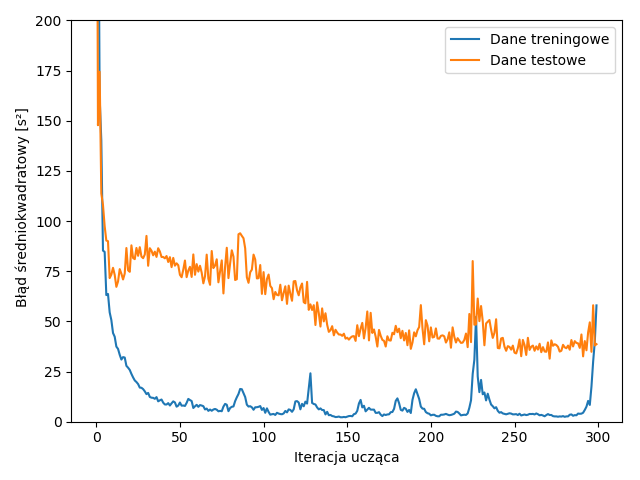
\includegraphics[width =\linewidth]{wykresy/6_regularyzacja/l1/regularyzacja_0_1_wykres_uczenia.png}
		 		\caption{parametr $\lambda$ - 0,1}
		 	\end{subfigure}
		 	\begin{subfigure}{.5\linewidth}
		 		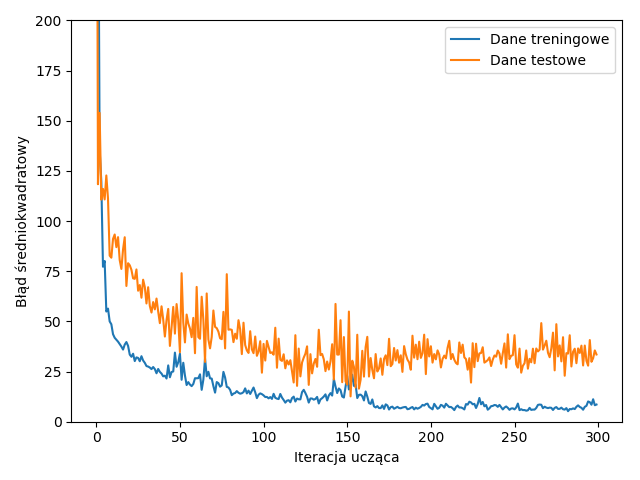
\includegraphics[width =\linewidth]{wykresy/6_regularyzacja/l1/regularyzacja_0_3_wykres_uczenia.png}
		 		\caption{parametr $\lambda$ - 0,3}
		 	\end{subfigure}
		 	
		 	\begin{subfigure}{.5\linewidth}
		 		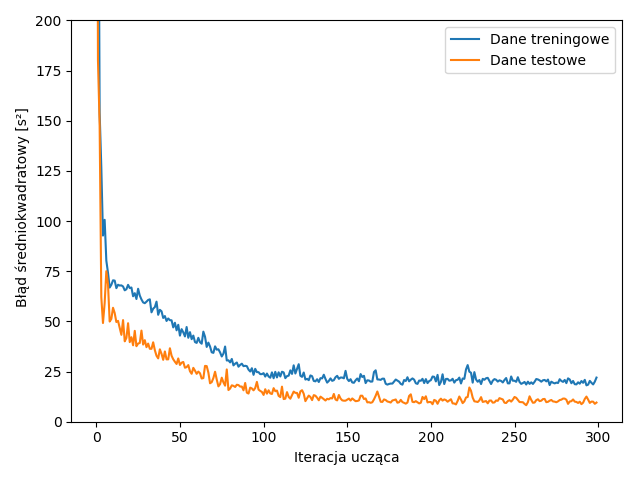
\includegraphics[width =\linewidth]{wykresy/6_regularyzacja/l1/regularyzacja_1_wykres_uczenia.png}
		 		\caption{parametr $\lambda$ - 1}
		 	\end{subfigure}
		 	\begin{subfigure}{.5\linewidth}
		 		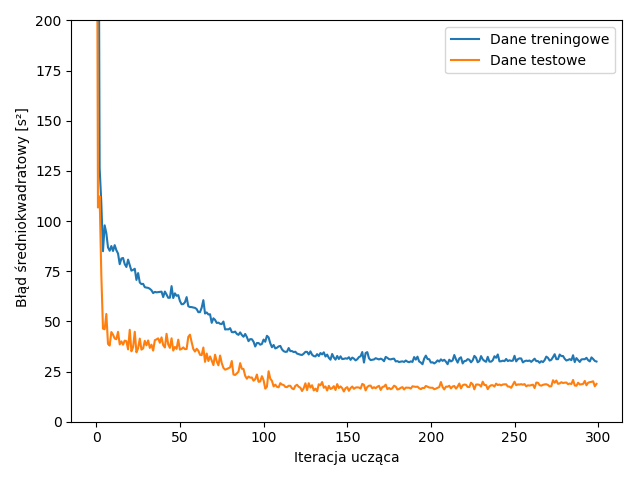
\includegraphics[width =\linewidth]{wykresy/6_regularyzacja/l1/regularyzacja_3_wykres_uczenia.png}
		 		\caption{parametr $\lambda$ - 3}
		 	\end{subfigure}
		  	
		  	\caption{Krzywe uczące dla najlepszych przypadków używając regularyzacji L1 w drugim modelu.}
			\label{fig: drugi_model_przy_regularyzacji_l1_wykresy_uczenia}
		\end{figure}
		 	
		 \begin{figure}[h]
		 	\begin{subfigure}{.5\linewidth}
		 		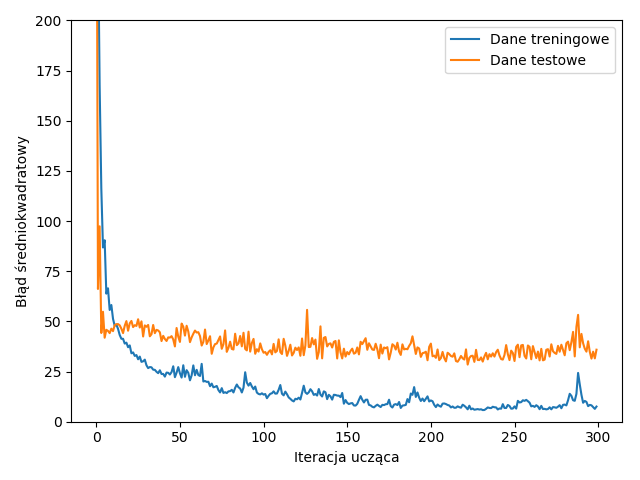
\includegraphics[width =\linewidth]{wykresy/6_regularyzacja/l2/regularyzacja_0_1_wykres_uczenia.png}
		 		\caption{parametr $\lambda$ - 0,1}
		 	\end{subfigure}
		 	\begin{subfigure}{.5\linewidth}
		 		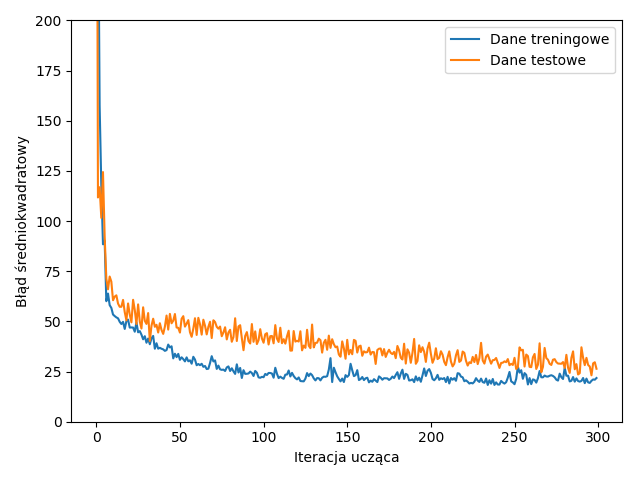
\includegraphics[width =\linewidth]{wykresy/6_regularyzacja/l2/regularyzacja_0_3_wykres_uczenia.png}
		 		\caption{parametr $\lambda$ - 0,3}
		 	\end{subfigure}
		 	
		 	\begin{subfigure}{.5\linewidth}
		 		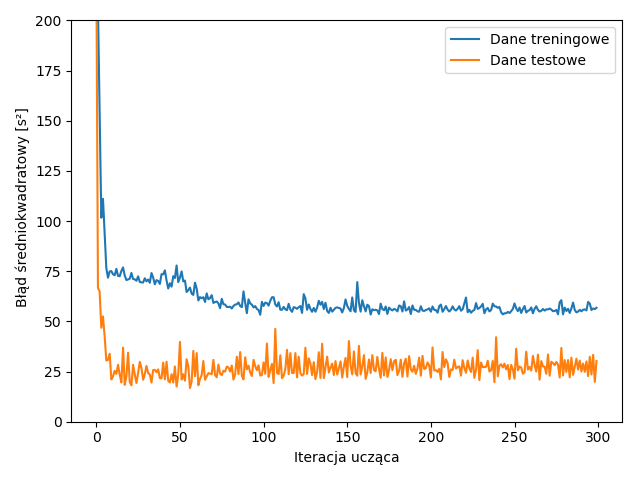
\includegraphics[width =\linewidth]{wykresy/6_regularyzacja/l2/regularyzacja_1_wykres_uczenia.png}
		 		\caption{parametr $\lambda$ - 1}
		 	\end{subfigure}
		 	\begin{subfigure}{.5\linewidth}
		 		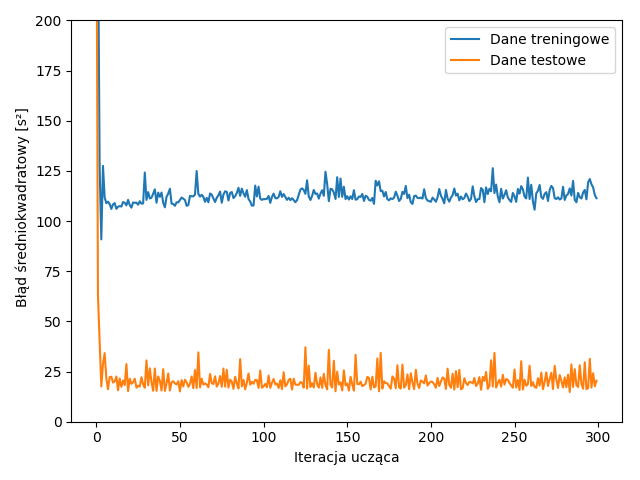
\includegraphics[width =\linewidth]{wykresy/6_regularyzacja/l2/regularyzacja_3_wykres_uczenia.png}
		 		\caption{parametr $\lambda$ - 3}
		 	\end{subfigure}
	 	
 			\caption{Krzywe uczące dla najlepszych przypadków używając regularyzacji L2 w drugim modelu.}
			\label{fig: drugi_model_przy_regularyzacji_l2_wykresy_uczenia}
		\end{figure}
		
		\begin{figure}[h]
			\begin{subfigure}{.5\linewidth}
		 		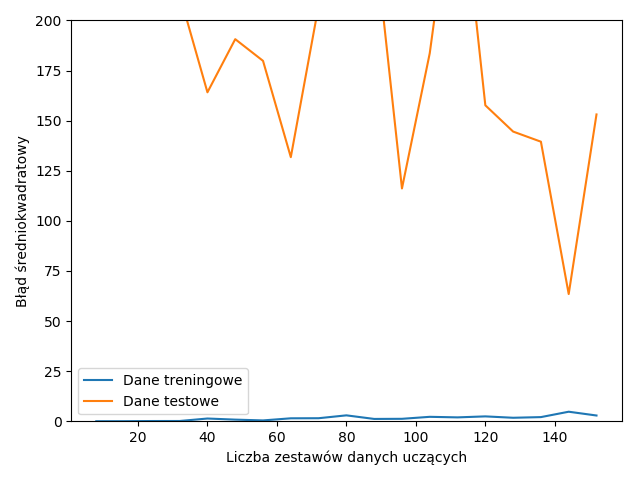
\includegraphics[width =\linewidth]{wykresy/6_regularyzacja/l1/regularyzacja_0_1_learning_curves.png}
		 		\caption{parametr $\lambda$ - 0,1}
		 	\end{subfigure}
		 	\begin{subfigure}{.5\linewidth}
		 		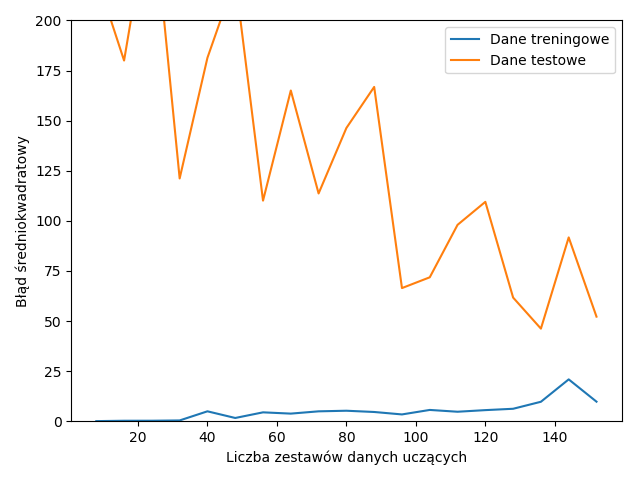
\includegraphics[width =\linewidth]{wykresy/6_regularyzacja/l1/regularyzacja_0_3_learning_curves.png}
		 		\caption{parametr $\lambda$ - 0,3}
		 	\end{subfigure}
		 	
		 	\begin{subfigure}{.5\linewidth}
		 		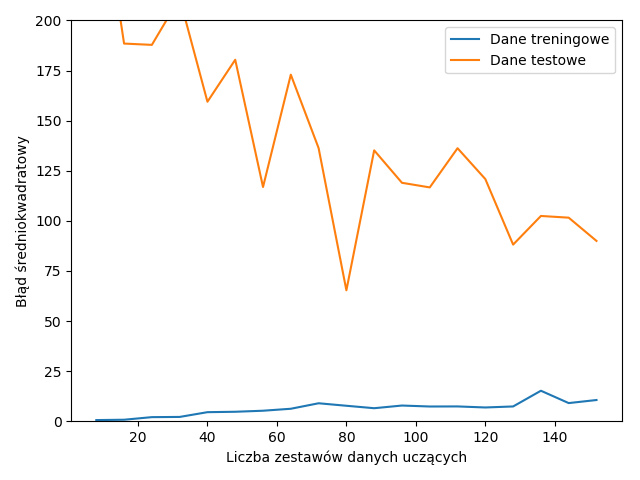
\includegraphics[width =\linewidth]{wykresy/6_regularyzacja/l1/regularyzacja_1_learning_curves.png}
		 		\caption{parametr $\lambda$ - 1}
		 	\end{subfigure}
		 	\begin{subfigure}{.5\linewidth}
		 		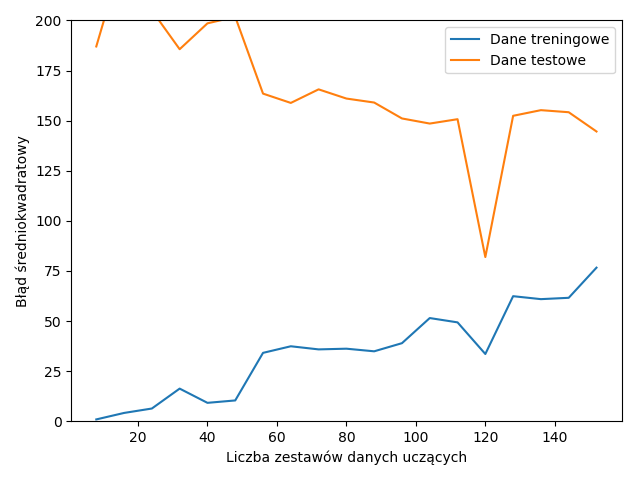
\includegraphics[width =\linewidth]{wykresy/6_regularyzacja/l1/regularyzacja_3_learning_curves.png}
		 		\caption{parametr $\lambda$ - 3}
		 	\end{subfigure}
		  	
		  	\caption{Krzywe uczące dla zmiennej ilości danych używając regularyzacji L1 w drugim modelu.}
			\label{fig: drugi_model_przy_regularyzacji_l1_learning_curves}
		\end{figure}
		 	
		 \begin{figure}[h]
		 	\begin{subfigure}{.5\linewidth}
		 		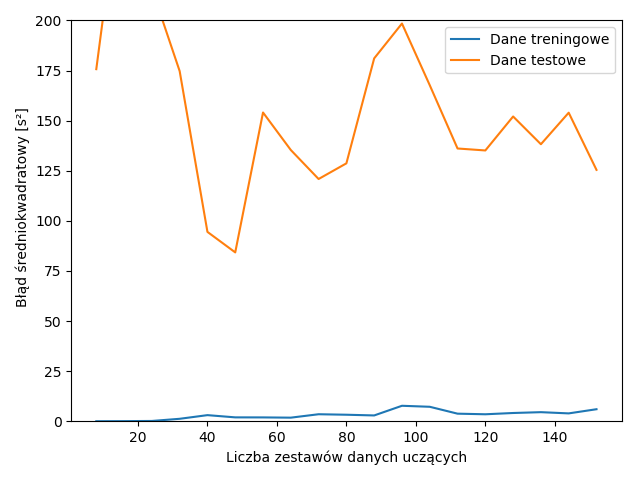
\includegraphics[width =\linewidth]{wykresy/6_regularyzacja/l2/regularyzacja_0_1_learning_curves.png}
		 		\caption{parametr $\lambda$ - 0,1}
		 	\end{subfigure}
		 	\begin{subfigure}{.5\linewidth}
		 		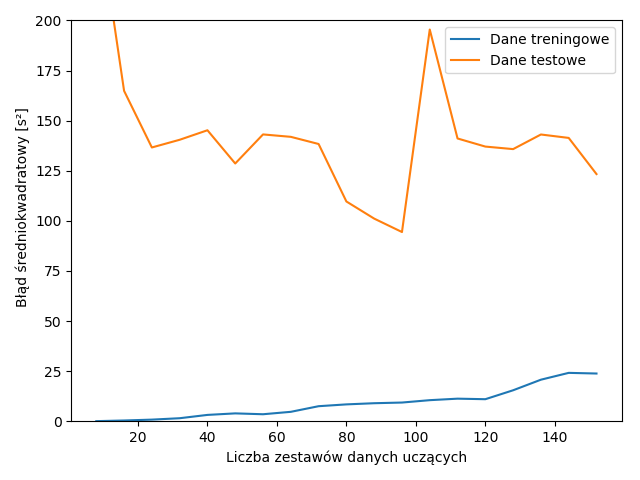
\includegraphics[width =\linewidth]{wykresy/6_regularyzacja/l2/regularyzacja_0_3_learning_curves.png}
		 		\caption{parametr $\lambda$ - 0,3}
		 	\end{subfigure}
		 	
		 	\begin{subfigure}{.5\linewidth}
		 		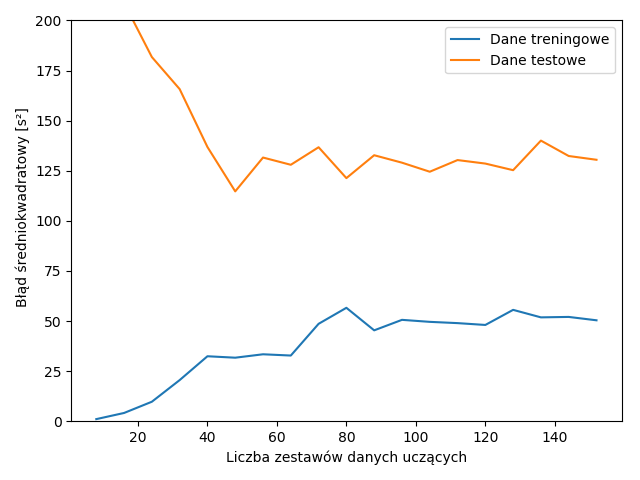
\includegraphics[width =\linewidth]{wykresy/6_regularyzacja/l2/regularyzacja_1_learning_curves.png}
		 		\caption{parametr $\lambda$ - 1}
		 	\end{subfigure}
		 	\begin{subfigure}{.5\linewidth}
		 		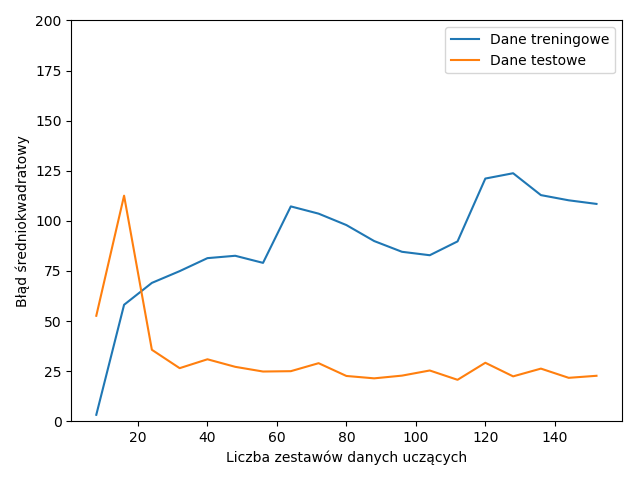
\includegraphics[width =\linewidth]{wykresy/6_regularyzacja/l2/regularyzacja_3_learning_curves.png}
		 		\caption{parametr $\lambda$ - 3}
		 	\end{subfigure}
	 	
 			\caption{Krzywe uczące dla zmiennej ilości danych używając regularyzacji L2 w drugim modelu.}
			\label{fig: drugi_model_przy_regularyzacji_l2_learning_curves}
		\end{figure}
		
		Po przeanalizowaniu wszystkich wykresów oraz wartości z tabeli nasunęły autor zanotował następujące spostrzeżenia:
		\begin{itemize}
		\item Bazując na tabeli, najlepsza kombinacja parametrów to funkcja regularyzacji \textit{L1} wraz z parametrem $\lambda$ równym 1. Przy tej kombinacji średni \textit{MSE} danych testowych jest najniższy oraz ma najniższe odchylenie.
		\item Patrząc na krzywe uczące dla najlepszych przypadków można zauważyć, że im wiekszy współczynnik $\lambda$, tym bardziej krzywa \textit{MSE} danych testowych ma tendencję do schodzenia poniżej krzywej \textit{MSE} danych treningowych. Oznacza to, że problem lepszego przewidywania danych ze zbioru testującego niż trenującego nie został wyeliminowany w całości. Widać także na nich, że dla $\lambda$, który w powyższym punkcie wydaje się najlepiej rokującą opcją, zdarzają się takie przypadki.
		\item Porównując krzywe uczące dla zmiennej ilości danych L1 z krzywymi L2, wśród tych pierwszych widać większą tendencję na zmniejszenie \textit{MSE} danych testowych przy większej ilości danych.
		\end{itemize}				
		
		Podsumowując, badając powyższe dane okazuje się, że uśrednianie danych nie wyeliminowało do końca problemu gorszego przyuczenia sieci do danych treningowych niż do testowych. Jednocześnie wstępnym wnioskiem na obecnych danych jest to, że regularyzacja \textit{L1} pomaga bardziej niż \textit{L2}. Jednakże aby mieć tego pewność, trzeba dokładniej sprawdzić dane oraz ewentualnie zebrać ich więcej, po czym zrobić powyższe testy jeszcze raz.
		
		\section{Badanie danych}
		Zastanawiającym problemem pojawiającym się w poprzednich rozdziałach było to, że często po nauczeniu sieci neuronowej, przewiduje ona dane testujące lepiej niż treningowe. Zwiększając poziom skomplikowania sieci neuronowej sytuacja się nie zmieniała, co dowiodło że ten problem leży nie po stronie modelu, a po stronie danych. Z tego powodu autor postanowił sprawdzić jakie wartości przyjmują dane wyjściowe w moim zbiorze danych. Autor wyrysował więc histogram obrazujący ilość danych dla danego czasu ewakuacji widoczny na rysunku \ref{fig: zaleznosc_ilosci_danych_od_czasu_ewakuacji}.
		
		\begin{figure}[h]
			\begin{tightcenter}
		 		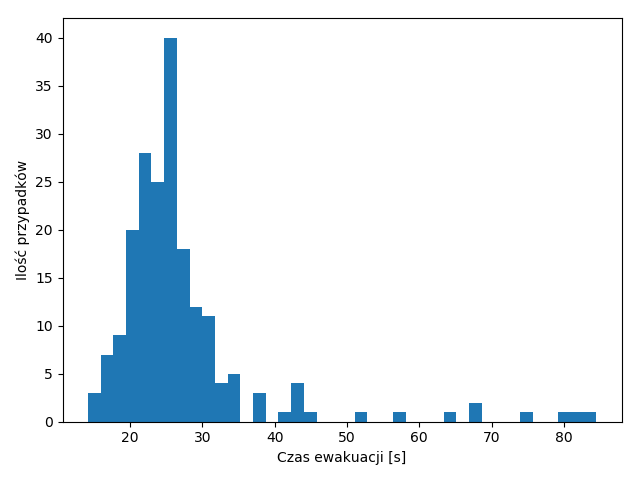
\includegraphics[width = 0.75\linewidth]{/home/xaaq/my-projects/inzynierka/inzynierka_latex/wykresy/7_badanie_danych/histogram_danych_czasu_ewakuacji.png}
		 	\end{tightcenter}
		 	
		  	\caption{Zależność ilości danych od czasu ewakuacji.}
			\label{fig: zaleznosc_ilosci_danych_od_czasu_ewakuacji}
		\end{figure}
		
		Analizując powyższy histogram widać, że większość danych wyjściowych jest skupiona poniżej 40 sekund czasu ewakuacji, a jedynie nieliczne wyniki przekraczają górną granicę. Taki rozrzut części danych może powodować, że będą one trudne do nauczenia przez model - autor postanowił więc odrzucić wszystkie zestawy danych, których dana wyjściowa - czas ewakuacji - jest równe lub większe 40 sekund. Po takiej operacji zostało 185 wektorów danych wejściowych i wyjsciowych. Na nich wykonane zostało badanie identyczne jak w sekcji \ref{regularyzacja_modelu}. Średnie wyniki autor umieścił w tabeli \ref{porownanie_srednich_wartosci_mse_po_odrzuceniu_czesci_danych}, krzywe uczenia dla najlepszych przypadków na rysunkach \ref{fig: drugi_model_przy_regularyzacji_l1_po_odrzuceniu_czesci_danych_wykresy_uczenia} i \ref{fig: drugi_model_przy_regularyzacji_l2_po_odrzuceniu_czesci_danych_wykresy_uczenia} oraz krzywe uczenia przy zmiennej ilości danych - na rysunkach \ref{fig: drugi_model_przy_regularyzacji_l1_po_odrzuceniu_czesci_danych_learning_curves} i \ref{fig: drugi_model_przy_regularyzacji_l2_po_odrzuceniu_czesci_danych_learning_curves}.
		
		\begin{table}[t]
			\caption{Porównanie średnich wartości \textit{MSE} danych po odrzuceniu części danych.}
			\begin{mytabular}{L L L c}
					Rodzaj regularyzacji & Ilość neuronów w warstwie & MSE danych treningowych & MSE danych testowych \\
					L1 & 0,1 & 4,13 ($\pm$0,65) & 15,63 ($\pm$3,32) \\
					L1 & 0,3 & 7,21 ($\pm$0,64) & 10,82 ($\pm$3,16) \\
					L1 & 1 & 10,45 ($\pm$0,49) & 9,35 ($\pm$2,73) \\
					L1 & 3 & 12,87 ($\pm$0,92) & 13,87 ($\pm$2,46) \\
					L2 & 0,1 & 4,31 ($\pm$1,58) & 12,97 ($\pm$3,42) \\
					L2 & 0,3 & 8,08 ($\pm$0,72) & 12,63 ($\pm$2,36) \\
					L2 & 1 & 11,63 ($\pm$0,76) & 12,97 ($\pm$3,12) \\
					L2 & 3 & 16,90 ($\pm$1,17) & 16,43 ($\pm$2,89)
			\end{mytabular}
			\label{porownanie_srednich_wartosci_mse_po_odrzuceniu_czesci_danych}
		\end{table}

		\begin{figure}[h]
			\begin{subfigure}{.5\linewidth}
		 		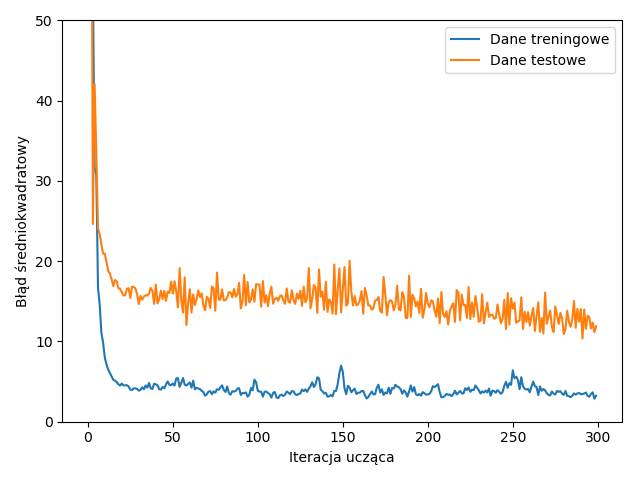
\includegraphics[width =\linewidth]{wykresy/7_badanie_danych/l1/regularyzacja_0_1_wykres_uczenia.png}
		 		\caption{parametr $\lambda$ - 0,1}
		 	\end{subfigure}
		 	\begin{subfigure}{.5\linewidth}
		 		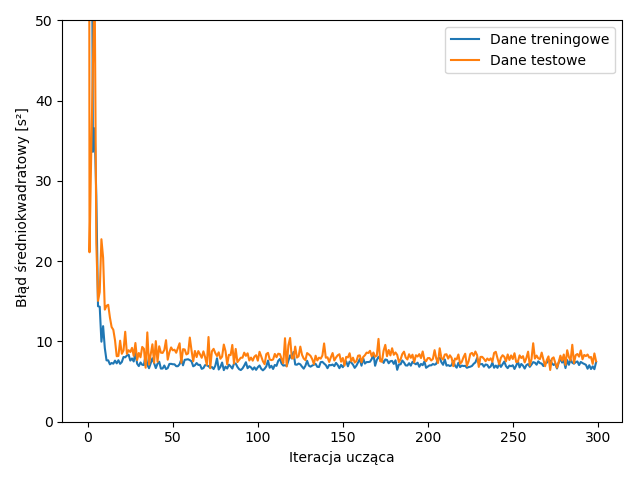
\includegraphics[width =\linewidth]{wykresy/7_badanie_danych/l1/regularyzacja_0_3_wykres_uczenia.png}
		 		\caption{parametr $\lambda$ - 0,3}
		 	\end{subfigure}
		 	
		 	\begin{subfigure}{.5\linewidth}
		 		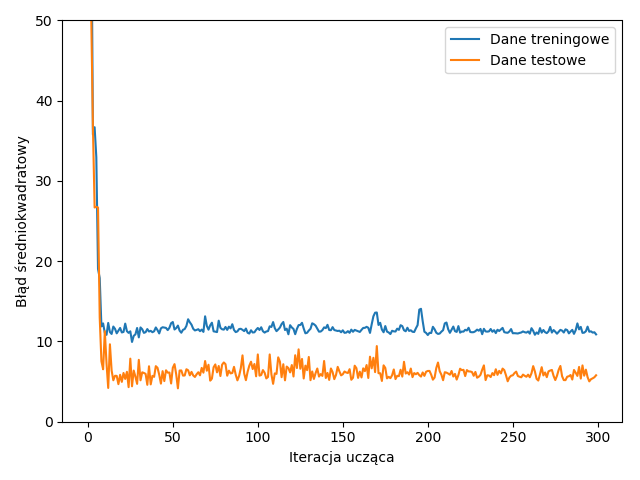
\includegraphics[width =\linewidth]{wykresy/7_badanie_danych/l1/regularyzacja_1_wykres_uczenia.png}
		 		\caption{parametr $\lambda$ - 1}
		 	\end{subfigure}
		 	\begin{subfigure}{.5\linewidth}
		 		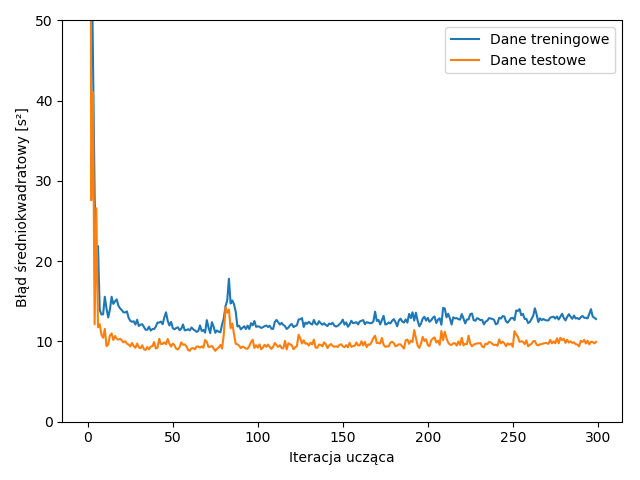
\includegraphics[width =\linewidth]{wykresy/7_badanie_danych/l1/regularyzacja_3_wykres_uczenia.png}
		 		\caption{parametr $\lambda$ - 3}
		 	\end{subfigure}
		  	
		  	\caption{Krzywe uczące dla najlepszych przypadków używając regularyzacji L1 w drugim modelu po odrzuceniu częsci danych.}
			\label{fig: drugi_model_przy_regularyzacji_l1_po_odrzuceniu_czesci_danych_wykresy_uczenia}
		\end{figure}
		 	
		\begin{figure}[h]
		 	\begin{subfigure}{.5\linewidth}
		 		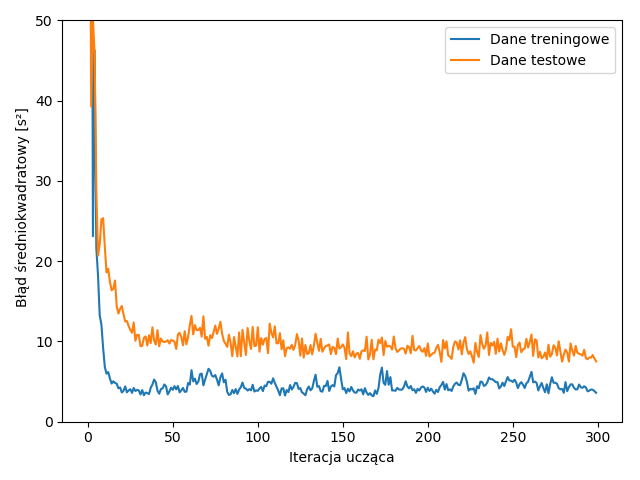
\includegraphics[width =\linewidth]{wykresy/7_badanie_danych/l2/regularyzacja_0_1_wykres_uczenia.png}
		 		\caption{parametr $\lambda$ - 0,1}
		 	\end{subfigure}
		 	\begin{subfigure}{.5\linewidth}
		 		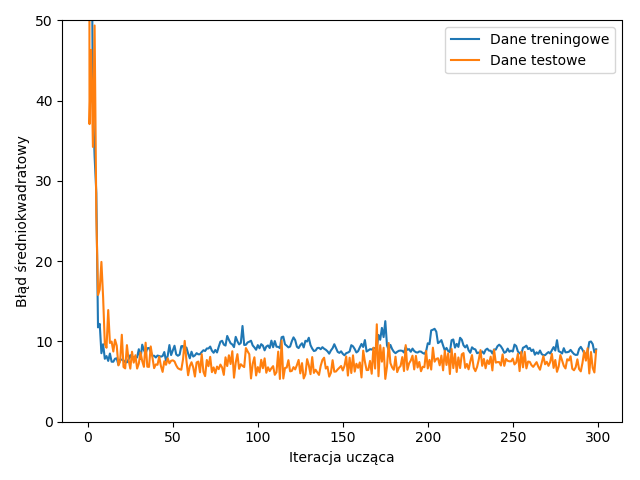
\includegraphics[width =\linewidth]{wykresy/7_badanie_danych/l2/regularyzacja_0_3_wykres_uczenia.png}
		 		\caption{parametr $\lambda$ - 0,3}
		 	\end{subfigure}
		 	
		 	\begin{subfigure}{.5\linewidth}
		 		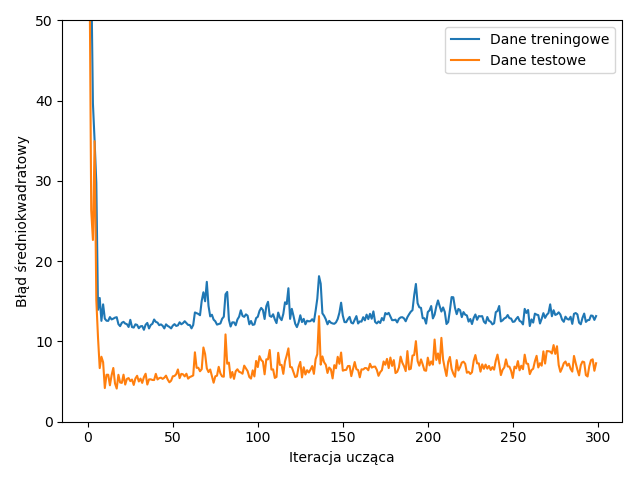
\includegraphics[width =\linewidth]{wykresy/7_badanie_danych/l2/regularyzacja_1_wykres_uczenia.png}
		 		\caption{parametr $\lambda$ - 1}
		 	\end{subfigure}
		 	\begin{subfigure}{.5\linewidth}
		 		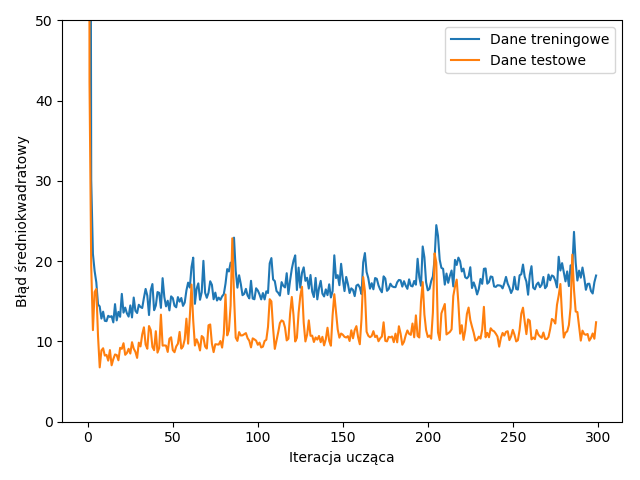
\includegraphics[width =\linewidth]{wykresy/7_badanie_danych/l2/regularyzacja_3_wykres_uczenia.png}
		 		\caption{parametr $\lambda$ - 3}
		 	\end{subfigure}
	 	
 			\caption{Krzywe uczące dla najlepszych przypadków używając regularyzacji L2 w drugim modelu po odrzuceniu częsci danych.}
			\label{fig: drugi_model_przy_regularyzacji_l2_po_odrzuceniu_czesci_danych_wykresy_uczenia}
		\end{figure}
		
		\begin{figure}[h]
			\begin{subfigure}{.5\linewidth}
		 		\includegraphics[width =\linewidth]{wykresy/7_badanie_danych/l1/regularyzacja_0_1_learning_curves.png}
		 		\caption{parametr $\lambda$ - 0,1}
		 	\end{subfigure}
		 	\begin{subfigure}{.5\linewidth}
		 		\includegraphics[width =\linewidth]{wykresy/7_badanie_danych/l1/regularyzacja_0_3_learning_curves.png}
		 		\caption{parametr $\lambda$ - 0,3}
		 	\end{subfigure}
		 	
		 	\begin{subfigure}{.5\linewidth}
		 		\includegraphics[width =\linewidth]{wykresy/7_badanie_danych/l1/regularyzacja_1_learning_curves.png}
		 		\caption{parametr $\lambda$ - 1}
		 	\end{subfigure}
		 	\begin{subfigure}{.5\linewidth}
		 		\includegraphics[width =\linewidth]{wykresy/7_badanie_danych/l1/regularyzacja_3_learning_curves.png}
		 		\caption{parametr $\lambda$ - 3}
		 	\end{subfigure}
		  	
		  	\caption{Krzywe uczące dla zmiennej ilości danych używając regularyzacji L1 w drugim modelu po odrzuceniu częsci danych.}
			\label{fig: drugi_model_przy_regularyzacji_l1_po_odrzuceniu_czesci_danych_learning_curves}
		\end{figure}
		 	
		\begin{figure}[h]
		 	\begin{subfigure}{.5\linewidth}
		 		\includegraphics[width =\linewidth]{wykresy/7_badanie_danych/l2/regularyzacja_0_1_learning_curves.png}
		 		\caption{parametr $\lambda$ - 0,1}
		 	\end{subfigure}
		 	\begin{subfigure}{.5\linewidth}
		 		\includegraphics[width =\linewidth]{wykresy/7_badanie_danych/l2/regularyzacja_0_3_learning_curves.png}
		 		\caption{parametr $\lambda$ - 0,3}
		 	\end{subfigure}
		 	
		 	\begin{subfigure}{.5\linewidth}
		 		\includegraphics[width =\linewidth]{wykresy/7_badanie_danych/l2/regularyzacja_1_learning_curves.png}
		 		\caption{parametr $\lambda$ - 1}
		 	\end{subfigure}
		 	\begin{subfigure}{.5\linewidth}
		 		\includegraphics[width =\linewidth]{wykresy/7_badanie_danych/l2/regularyzacja_3_learning_curves.png}
		 		\caption{parametr $\lambda$ - 3}
		 	\end{subfigure}
	 	
 			\caption{Krzywe uczące dla zmiennej ilości danych używając regularyzacji L2 w drugim modelu po odrzuceniu częsci danych.}
			\label{fig: drugi_model_przy_regularyzacji_l2_po_odrzuceniu_czesci_danych_learning_curves}
		\end{figure}		
		
		Badając powyższe wykresy nasuwają się następujące wnioski:
		\begin{itemize}
		\item Odrzucenie przypadków skrajnie odstających od reszty obniżyło \textit{MSE} danych co najmniej 3-krotnie (a w dotychczas najgorszych przypadkach nawet 10-krotnie), co daje jednoznaczną odpowiedź gdzie leżał problem z lepszym przyuczeniem sieci do danych testowych.
		\item Analizując tabelę \ref{porownanie_srednich_wartosci_mse_po_odrzuceniu_czesci_danych} wygląda na to, że tak jak poprzednio - funkcja regularyzacji \textit{L1} z parametrem $\lambda$ równym \textbf{1} daje najlepsze rezultaty. Jeznakże nie wiele gorszym zestawem parametrów, ze zbliżonym \textit{MSE} danych testowych odznacza się ta sama funkcja z parametrem $\lambda$ równym \textbf{0,3}.
		\item Patrząc na wykresy krzywych uczących dla najlepszych przypadków widać, że niezależnie czy użyta została funkcja regularyzacji \textit{L1} czy \textit{L2}, przy parametrze $\lambda$ równym \textbf{1} sieć przyucza się minimalnie lepiej do danych testowych. Pamiętając co było źródłem dotychczasowego problemu można wywnioskować, że takie zachowanie może być spowodowane przez szumy zbioru danych, a sposobem ich wyeliminowania było by zebranie danych z większej ilości symulacji przeprowadzonych z wyższym parametrem \textit{Repeat number}.
		\end{itemize}
		
		Podsumowując, w wyniku przeprowadzonych badań została znaleziony najlepsze kombinacje parametrów regularyzacji dla obecnych danych - funkcja \textit{L1} z parametrem $\lambda$ równym \textbf{0,3} lub \textbf{1}. Jednakże istnieje podejrzenie, że przez niską ilość powtórzeń symulacji dla danego zestawu parametrów wejściowych, w zbiorze danych wyjściowych istnieją szumy, których eliminacja podniosłaby efektywność sieci przy parametrze $\lambda$ równym \textbf{1}.
		
		\section{Zebranie większej ilości danych}	
		Chcąc zbadać hipotezę, że przy parametrze regularyzacji $\lambda$ równym 1 model będzie się uczył lepiej na wiekszej ilości danych, autor postanowił powtórzyć proces generacji danych symulacyjnych. Zrobione zostało to podobnie jak w sekcji \ref{zebranie_danych} z tym, że parametr \textit{Repeat number} w wygenerowanych plikach ustawiony na 50. Dzięki temu każda dana wyjściowa powinna być stabilniejsza ze względu na obliczanie średniej na 5 razy wiekszej liczbie przypadków niż dotychczas.
		
		Po zebraniu danych oraz uśrednieniu ich w taki sam sposób jak w sekcji \ref{usrednianie_danych} powiększyłem zbiór uczący o kolejne 200 przypadków. Postanowiłem przeprowadzić badanie, jak wpłynie na model nauka na:
		\begin{itemize}
		\item \textbf{zestawie danych numer 1} - danych zebranych w sekcji \ref{zebranie_danych},
		\item \textbf{zestawie danych numer 2} - danych zebranych w tej sekcji,
		\item \textbf{zestawie danych numer 3} - połączonym zestawie danych numer 1 i 2.
		\end{itemize}
		W eksperymencie sieć została osobno nauczona dla każdej kombinacji wielkości zbioru danych uczących oraz parametrów uczenia $\lambda$ - \textbf{0,3} i \textbf{1}.
		
		Wyniki eksperymentów są następujące:
		\begin{itemize}
		\item porównanie średnich wartości \textit{MSE} danych w tabeli \ref{porownanie_srednich_wartosci_mse_po_zebraniu_wiekszej_ich_ilosci},
		\item krzywe uczące dla najlepszych przypadków na rysunku \ref{fig: drugi_model_po_zebraniu_wiekszej_ilosci_danych_wykresy_uczenia},
		\item krzywe uczące dla zmiennej ilości danych na rysunku \ref{fig: drugi_model_po_zebraniu_wiekszej_ilosci_danych_learning_curves}.
		\end{itemize}						
		
		\begin{table}[t]
			\caption{Porównanie średnich wartości \textit{MSE} danych po zebraniu większej ich ilości.}
			\begin{mytabular}{L L L L}
					Zestaw danych & Parametr regularyzacji L1 & MSE danych treningowych & MSE danych testowych \\
					stary & 0,3 & 7,02 ($\pm$0,56) & 11,58 ($\pm$4,83) \\
					stary & 1 & 10,51 ($\pm$0,85) & 9,50 ($\pm$2,87) \\
					nowy & 0,3 & 10,76 ($\pm$0,88) & 19,48 ($\pm$3,95) \\
					nowy & 1 & 14,53 ($\pm$1,10) & 14,90 ($\pm$5,51) \\
					stary + nowy & 0,3 & 14,72 ($\pm$0,65) & 14,23 ($\pm$2,16) \\
					stary + nowy & 1 & 14,80 ($\pm$0,98) & 15,94 ($\pm$3,00) \\
			\end{mytabular}
			\label{porownanie_srednich_wartosci_mse_po_zebraniu_wiekszej_ich_ilosci}
		\end{table}	
		
		\begin{figure}[h]
			\begin{subfigure}{.5\linewidth}
		 		\includegraphics[width =\linewidth]{wykresy/8_zebranie_wiekszej_ilosci_danych/0-200/regularyzacja_0_3_wykres_uczenia.png}
		 		\caption{stary zestaw danych, parametr $\lambda$ - 0,3}
		 	\end{subfigure}
		 	\begin{subfigure}{.5\linewidth}
		 		\includegraphics[width =\linewidth]{wykresy/8_zebranie_wiekszej_ilosci_danych/0-200/regularyzacja_1_wykres_uczenia.png}
		 		\caption{stary zestaw danych, parametr $\lambda$ - 1}
		 	\end{subfigure}
		
		 	\begin{subfigure}{.5\linewidth}
		 		\includegraphics[width =\linewidth]{wykresy/8_zebranie_wiekszej_ilosci_danych/200-400/regularyzacja_0_3_wykres_uczenia.png}
		 		\caption{nowy zestaw danych, parametr $\lambda$ - 0,3}
		 	\end{subfigure}
		 	\begin{subfigure}{.5\linewidth}
		 		\includegraphics[width =\linewidth]{wykresy/8_zebranie_wiekszej_ilosci_danych/200-400/regularyzacja_1_wykres_uczenia.png}
		 		\caption{nowy zestaw danych, parametr $\lambda$ - 1}
		 	\end{subfigure}
		 	
		 	\begin{subfigure}{.5\linewidth}
		 		\includegraphics[width =\linewidth]{wykresy/8_zebranie_wiekszej_ilosci_danych/0-400/regularyzacja_0_3_wykres_uczenia.png}
		 		\caption{oba zestawy danych, parametr $\lambda$ - 0,3}
		 	\end{subfigure}
		 	\begin{subfigure}{.5\linewidth}
		 		\includegraphics[width =\linewidth]{wykresy/8_zebranie_wiekszej_ilosci_danych/0-400/regularyzacja_1_wykres_uczenia.png}
		 		\caption{oba zestawy danych, parametr $\lambda$ - 1}
		 	\end{subfigure}
	 	
 			\caption{Krzywe uczące dla najlepszych przypadków w drugim modelu po zebraniu większej ilości danych.}
			\label{fig: drugi_model_po_zebraniu_wiekszej_ilosci_danych_wykresy_uczenia}
		\end{figure}
		
		\begin{figure}[h]
			\begin{subfigure}{.5\linewidth}
		 		\includegraphics[width =\linewidth]{wykresy/8_zebranie_wiekszej_ilosci_danych/0-200/regularyzacja_0_3_learning_curves.png}
		 		\caption{stary zestaw danych, parametr $\lambda$ - 0,3}
		 	\end{subfigure}
		 	\begin{subfigure}{.5\linewidth}
		 		\includegraphics[width =\linewidth]{wykresy/8_zebranie_wiekszej_ilosci_danych/0-200/regularyzacja_1_learning_curves.png}
		 		\caption{stary zestaw danych, parametr $\lambda$ - 1}
		 	\end{subfigure}
		
		 	\begin{subfigure}{.5\linewidth}
		 		\includegraphics[width =\linewidth]{wykresy/8_zebranie_wiekszej_ilosci_danych/200-400/regularyzacja_0_3_learning_curves.png}
		 		\caption{nowy zestaw danych, parametr $\lambda$ - 0,3}
		 	\end{subfigure}
		 	\begin{subfigure}{.5\linewidth}
		 		\includegraphics[width =\linewidth]{wykresy/8_zebranie_wiekszej_ilosci_danych/200-400/regularyzacja_1_learning_curves.png}
		 		\caption{nowy zestaw danych, parametr $\lambda$ - 1}
		 	\end{subfigure}
		 	
		 	\begin{subfigure}{.5\linewidth}
		 		\includegraphics[width =\linewidth]{wykresy/8_zebranie_wiekszej_ilosci_danych/0-400/regularyzacja_0_3_learning_curves.png}
		 		\caption{oba zestawy danych, parametr $\lambda$ - 0,3}
		 	\end{subfigure}
		 	\begin{subfigure}{.5\linewidth}
		 		\includegraphics[width =\linewidth]{wykresy/8_zebranie_wiekszej_ilosci_danych/0-400/regularyzacja_1_learning_curves.png}
		 		\caption{oba zestawy danych, parametr $\lambda$ - 1}
		 	\end{subfigure}
	 	
 			\caption{Krzywe uczące dla zmiennej ilości danych w drugim modelu po zebraniu większej ich ilości.}
			\label{fig: drugi_model_po_zebraniu_wiekszej_ilosci_danych_learning_curves}
		\end{figure}
		
		Po analizie danych autor doszedł do następujących wniosków:
		\begin{itemize}
		\item Wbrew oczekiwaniom - na zbiorze numer 1 danych sieć neuronowa dawała lepsze rezultaty, w najlepszym przypadku - mniejsze o około 5 sekund kwadratowych od wyników na pozostałych zbiorach.
		\item Co jest niespodziewane - na zbiorze numer 2 (teoretycznie stabilniejszych danych) sieć miała największe problemy z nauką osiągając nawet dwukrotnie wyższe średnie lub odchylenia \textit{MSE} danych testowych w stosunku do najlepszych przypadków.
		\item Na wykresach krzywych uczących dla najlepszych przypadków widać, że nie ważne z jakiego zbioru danych sieć korzystała, to i tak czasami pojawiają się szumy powodujące lepsze przyuczenie sieci do danych testowych.
		\item Analiza wykresów krzywych uczących dla zmiennej ilości danych obrazują jak ilość danych wpłynęła na \textit{MSE} danych - dopiero większa ilość danych sprawiła, że krzywe danych treningowych i testowych zetknęły się ze sobą - oznacza to większą stabilność przewidywania danych co jest cechą bardzo porządaną.
		\end{itemize}	
		
		Zbiór danych numer 2 tylko pogorszył \textit{MSE} modelu; podobny efekt dał zbiór danych numer 3. Obaliło to tezę, jako że większy zestaw danych miałby zmniejszyć ich \textit{MSE}. Jednakże zestaw danych numer 3 wprowadził do modelu większą stabilność, co przełożyło się na bardziej do siebie zbliżony średni \textit{MSE} danych testowych oraz danych treningowych. Szczególnie jest to prawdą dla parametru $\lambda$ równego \textbf{0,3} - oznacza to, że do osiągnięcia największej stabilności modelu o akceptowalnym poziomie \textit{MSE} właśnie on będzie dalej używany. Jeśli chodzi o zbiór uczący - do dalszego użytku został wybrany zbiór numer 3.
		
		\section{Podsumowanie}	
		Podsumowując, po procesie dostrajania parametrów sieci neuronowej udało się osiągnąć model, mający błąd średniokwadratowy około 15 s$^2$. Parametry ostatecznego modelu sieci neuronowej były następujące:
		\begin{itemize}
		\item 1 warstwa ukryta z 20 neuronami i funkcją aktywacji ReLU,
		\item warstwa wyjściowa składająca się z jednego neuronu z funkcją aktywacji ReLU,
		\item użyta \textbf{regularyacja L1} ze współczynnikiem $\lambda$ równym \textbf{0,3},
		\item \textbf{współczynnik uczenia} - 0.1,
		\item \textbf{metryka do optymalizacji} - MSE,
		\item \textbf{liczba epok uczacych} - 300,
		\item podział na \textbf{dane treningowe} i \textbf{dane testowe} - 80\% : 20\%.
		\end{itemize}
		
		Operacje wykonane na danych uczących przed rozpoczęciem procesu uczącego były następujące:
		\begin{enumerate}
		\item uśrednienie wszystkich powtórzeń pojedynczej symulacji,
		\item odrzucenie wszystkich zestawów danych, których dana wyjściowa (czas ewakuacji) była większa lub równa 40,
		\item normalizacja danych opisana w sekcji \ref{normalizacja_danych}.		
		\end{enumerate}
		
		Na koniec strzowone zostało 20 modeli z powyższymi parametrami, które zostały osobno uczone. Po zakończeniu procesu nauki do dalszych badań autor wybrał ten, który miał najmniejszą różnicę pomiędzy błędem na danych treningowych i na danych testowych.
		
	\chapter{Optymalizacja modelu}
	\textit{W tym rozdziale opisany zostanie proces optymalizacji wyjść modelu na podstawie danych wejściowych.}

		\section{Proces optymalizacji modelu}
		Algorytmem optymalizacji użytym przez autora była \textit{metoda gradientu prostego} opisana w sekcji \ref{optymalizacja_wyjsc_modelu}. Sam proces był następujący:
		\begin{enumerate}
		\item Weź jeden losowo wybrany zestaw danych ze zbioru.
		\item Jeśli dana wyjściowa tego zestawu jest większa od 40, wróć do punktu 1.
		\item Znormalizuj dane wejściowe.
		\item Wykonaj 100 iteracji algorytmu \textit{Gradient descent} w celu optymalizacji wyjścia modelu na podstawie jego wejść, przy czym wejścia nie mogą wykroczyć poza ustalony przez twórców symulatora \textit{PSP} zakres (na przykład aby nie dostać negatywnej liczby pieszych w symulacji).
		\item Wykonaj de-normalizacje danych wejściowych i zapisz je do pliku \textit{.xml} z parametrem powtórzeń \textit{Repeat number} ustawionym na 10.
		\item Wykonaj symulacje na podstawie zapisanych danych.
		\item Oblicz średnią daną wyjściową ze wszystkich symulacji.
		\end{enumerate}
		
		Powyższy proces wykonany został 10 razy a jego wyniki są widoczne w tabeli \ref{porownanie_rzeczywistych_i_przewidywanych_czasow_symulacji_przed_i_po_optymalizacji}. W pierwszej i drugiej kolumnie widać rzeczywiste i przewidziane przez model czasy ewakuacji - różnią się one nieznacznie, lecz w granicach błędu uczenia widocznego na wykresach \ref{fig: drugi_model_po_zebraniu_wiekszej_ilosci_danych_wykresy_uczenia} i \ref{fig: drugi_model_po_zebraniu_wiekszej_ilosci_danych_learning_curves} (dla obu zestawów danych i parametru $\lambda$ równego 0,3). W trzeciej i czwartej kolumnie widoczne są czasy ewakuacji po procesie optymalizacji. Od razu widać, że wartości przewidziane przez model są prawie identyczne - oznacza to, że algorytm \textit{Gradient descent} prawidłowo znajduje minimum modelu, które nie zależy od tego z jakim zestawem danych rozpoczniemy optymalizację. Porównując kolumnę 3 i 4 można zauważyć, że dane rzeczywiste też mieszczą się w zakresie błędu uczącego; co więcej - w większości są one mniejsze od przewidywanego czasu ewakuacji o 1,5 - 2 sekund.
		
		\begin{table}[t]
			\caption{Porównanie rzeczywistych i przewidzianych czasów ewakuacji przed i po optymalizacji.}
			\begin{mytabular}{L L L L}
					Rzeczywisty czas ewakuacji przed optymalizacją [s] & Przewidywany czas ewakuacji przed optymalizacją [s] & Rzeczywisty czas ewakuacji po optymalizacji [s] & Przewidywany czas ewakuacji po optymalizacji [s] \\
					24.22 & 26.37 & 15.925 & 19.58 \\ 
				    23.27 & 22.11 & 18.125 & 19.57 \\ 
				    19.70 & 23.69 & 18.125 & 19.57 \\ 
				    26.12 & 24.43 & 17.475 & 19.57 \\ 
				    27.06 & 27.04 & 17.725 & 19.57 \\ 
				    22.39 & 27.72 & 17.45 & 19.57 \\ 
				    24.38 & 26.45 & 18.125 & 19.57 \\ 
				    23.98 & 27.48 & 17.875 & 19.57 \\ 
				    32.77 & 27.84 & 17.1625 & 19.59 \\ 
				    25.23 & 24.47 & 16.825 & 19.60
			\end{mytabular}
			\label{porownanie_rzeczywistych_i_przewidywanych_czasow_symulacji_przed_i_po_optymalizacji}
		\end{table}

		\section{Podsumowanie}
		Podsumowując, udało się przeprowadzić optymalizację wyjść modelu za pomocą algorytmu \textit{Gradient descent}. Przy każdej próbie czas ewakuacji był optymalizowany do prawie identycznych wartości co oznacza, że proces optymalizacji nie zależy od wartości początkowych. Porównując wartości wartości rzeczywiste i przewidywane przez model (przed jak i po optymalizacji), zdecydowana ich większość była w granicach błędu uczenia. Jak widać najniższy przewidywany przez sieć czas ewakuacji jest to 19,57 sekund - co po weryfikacji w symulatorze \textit{PSP} daje czasy w okolicach 17 - 18 sekund.
		
	\chapter{Podsumowanie}
	\textit{W tym rozdziale zostały podsumowane prace związane ze zbieraniem danych, budowaniem modelu i dostrajaniem jego parametrów. Znajduje się tu także podsumowanie procesu optymalizacji.}	
	
		\section{Podsumowanie procesu zbierania danych}
		Jako że w dziedzinie uczenia maszynowego operacje na danych są tak samo ważne jak budowa odpowiedniego modelu to i tym razem dane, które zostały zebrane z symulatora \textit{PSP} wymagały bliższego poznania i ewentualnej obróbki. Zbiór danych został poddany następującym operacjom:
		\begin{enumerate}
		\item uśrednienie wszystkich powtórzeń pojedynczej symulacji,
		\item odrzucenie wszystkich zestawów danych, których dana wyjściowa była większa lub równa 40,
		\item normalizacja danych.		
		\end{enumerate}
		
		Zbiór za pomocą którego autor uczył model miał 400 zestawów danych; dało to większą stabilność przewidywanych wyników w stosunku do zbioru składającego się z 200 zestawów danych. Jednakże mimo tego, nie wyeliminowało to zupełnie szumu związanego z czynnikami losowymi w symulatorze \textit{PSP}.
		
		\section{Podsumowanie budowy modelu}
		Budowa modelu była najdłuższą częścią projektu - wymagała ona dużej ilości testów z różnymi kombinacjami parametrów (gdzie niektóre z nich wykonywały się po kilka godzin). Ostatecznie udało się osiągnąć model, którego błąd średniokwadratowy był oscylował w granicach 15s$^2$. Wybranym modelem została sieć neuronowa z następującymi parametrami:
		\begin{itemize}
		\item 1 warstwa ukryta z 20 neuronami i funkcją aktywacji ReLU,
		\item warstwa wyjściowa składająca się z jednego neuronu z funkcją aktywacji ReLU,
		\item użyta \textbf{regularyacja L1} ze współczynnikiem $\lambda$ równym \textbf{0,3},
		\item \textbf{współczynnik uczenia} - 0.1,
		\item \textbf{metryka do optymalizacji} - MSE,
		\item \textbf{liczba epok uczacych} - 300,
		\item podział na \textbf{dane treningowe} i \textbf{dane testowe} - 80\% : 20\%.
		\end{itemize}
		
		Budowa takiego modelu pozwoliła uniezależnić się od symulatora \textit{PSP} podczas procesu symulacji - co było dużym zyskiem, gdyż symulacje trzeba było w nim włączać ręcznie.
		
		\section{Optymalizacja wyjść modelu}
		Ostatnią częścią projektu była optymalizacja danych wyjściowych modelu na podstawie jego wejść. Autor użył do tego algorytmu \textit{Gradient descent} z 10 różnymi zestawami danych do optymalizacji, co miało dać szerszy pogląd na to czy proces optymalizacji będzie generował duże szumy. Jak się okazało - model przewidywał daną wyjściową na podstawie danych wejściowych z wypracowaną wcześniej dokładnością, co było dobrym znakiem. Co więcej algorytm potrafił zoptymalizować wejścia modelu tak, żeby za każdym zwracał bardzo zbliżone wyniki. Daje to także ostateczne rozwiązanie postawionego problemu optymalnego wyboru ścieżki lub wyjścia ewakuacyjnego - dzięki odpowiedniemu dostrojeniu parametrów pieszych - szybkości, sposobu wyboru ścieżki, dozwolonej gęstości na metr kwadratowy i tym podobnch - udało się zminimalizować czas potrzebny na ich ewakuację. Czas jaki się udało osiągnąć było to przewidywane przez sieć - 19,57 sekund, a przetestowane w symulatorze - 17 - 18 sekund.
		
	\printbibliography
\end{document}
